The normalisation of the $t\bar{t}$ background is estimated 
from data as included as freely floating parameter in the final fit. 
This normalisation is correlated across all regions included in the fit and it is determined mainly from the tails of the $m_{\ell\ell}$ distribution in the dilepton CR which have high purity of \ttbar events.
%This normalisation is determined from the low PNN region of the $\tau_{lep}\tau_{had}$ 
%SLT signal region which is dominated by $t\bar{t}$ events.

Relative acceptance uncertainties on the normalisation are applied on 
\ttbar in the SRs
%$t\bar{t}$ in the other regions included in the fit, 
%the $\tau_{lep}\tau_{had}$ LTT signal region, 
%the $\tau_{had}\tau_{had}$ signal region and the Z+HF control region, 
to take into account potential differences in the normalisation 
between the SRs and the CR. 

In each signal region also shape variations are checked 
and applied, correlated with the relative acceptance uncertainties on the normalisations, where they are found to be relevant as described in the following. 

All these uncertainties are derived by MC-to-MC comparison, 
as described in Section~\ref{sec:systematics_backgroundmodelling}, 
following the 
\href{https://twiki.cern.ch/twiki/bin/view/AtlasProtected/TopMCSystematicsR21}{\underline{recommendations of the Top modelling group}}. 

Uncertainties due to PDF, $\alpha_s$, FSR and scales 
are evaluated using internal alternative weights present in all the $t\bar{t}$ nominal samples. 

Uncertainties from the parton shower, 
matrix element and ISR are estimated using 
the differences between the nominal samples and 
the corresponding variations samples, as reported in Table~\ref{sec:systs:tab:systematics_ttbar}. 
Parton shower hadronisation algorithmic uncertainties 
are evaluated comparing the nominal samples showered with Pythia8 
to alternative samples showered with Herwig7. 
ME NLO matching uncertainty is evaluated comparing 
the nominal Powheg+Pythia8 samples to alternative aMcAtNlo+Pythia8 samples. 
ISR up variation is evaluated by comparing the 
fast simulation nominal Powheg+Pythia8 (hdamp=1.5 mtop) with 
the fast simulation samples with varied hdamp (hdamp=3 mtop), 
at the same time dividing by 2 the renormalization 
and factorization scales and the varying the showering (Var3c Up); 
while the ISR down variation is evaluated by comparing 
the nominal Powheg+Pythia8 with the samples obtained 
doubling the renormalization and factorization scales and the varying the showering (Var3c Down).


\begin{table}
  \centering
  \begin{tabular}{|c|c|c|}
  \hline
  Source & DSID & Name\\
  \hline

  ME & 410464, 410465, 410466 &PhPy8EG\_A14\_ttbar\_hdamp258p75 \\
  PS & 410557, 410558, 410559   &aMcAtNloPy8EvtGen\_MEN30NLO\_A14N23LO\_ttbar\_noShWe \\
  ISR &410480, 410481, 410482  &PhPy8EG\_A14\_ttbar\_hdamp517p5 \\
   
  \hline
  \end{tabular}
  \caption{List of alternative \ttbar\ samples for PS, ME, ISR uncertainties.}
  \label{sec:systs:tab:systematics_ttbar}
  \end{table}
  


Relative acceptance uncertainties on the normalisation between the CR and the SRs
are calculated from the single channel acceptances using Equation~\ref{eq:relative_acceptance_unc} 
and are found in the different fit regions to be as large as reported in Table~\ref{sec:systs:tab:systematics_normalisations_ttbar}.


%Old ones from Lephad SLT SR to other regions
%\begin{table}
%\centering
%\small
%\begin{tabular}{|c|c|c|c|}
%\hline
%Source & Size in LepHad LTT SR & Size in HadHad SR & Size in Z+HF CR\\
%\hline
%ME & 0.016 & 0.035 & 0.0026\\
%PS & 0.015 &  0.047 & 0.067\\
%ISR & +0.021, -0.0056 & +0.0052, 0.0007 & +0.0082, -0.0005 \\
%FSR & -0.022, -0.0045 & +0.0051, -0.035 & +0.0098, -0.014\\
%PDF+$\alpha_s$ & 0.0014 & 0.0065 & 0.0059 \\
%Total & +0.028, -0.020 & +0.059, -0.068 & +- 0.069\\
%\hline
%\end{tabular}
%\caption{Relative acceptance normalisation uncertainties on $t\bar{t}$ for the di-Higgs analysis.}
%\label{sec:systs:tab:systematics_normalisations_ttbar}
%\end{table}

%New ones from CR to SRs
\begin{table}
\centering
\small
\begin{tabular}{|c|c|c|c|}
\hline
Source & Size in LepHad SLT & Size in LepHad LTT & Size in HadHad\\
\hline
ME & +0.0026, -0.0026 & -0.009, +0.009 & +0.037, -0.037\\
PS & -0.072, +0.072 & -0.088, +0.088 & -0.022, +0.022\\
ISR & +0.0005, -0.0081 & -0.0052, +0.013 & -0.0002, -0.003\\
FSR & +0.014, -0.0097 & +0.0096, -0.032 & +0.019, -0.045\\
PDF+$\alpha_s$ & -0.006, +0.006 & -0.0073, +0.0073 & -0.0011, +0.0011\\
Total & -0.074, +0.074 & -0.094, +0.090 & -0.062, +0.047\\
\hline
\end{tabular}
\caption{Relative size of relative acceptance normalisation uncertainties on $t\bar{t}$ for the di-Higgs analysis.}
\label{sec:systs:tab:systematics_normalisations_ttbar}
\end{table}


\paragraph{Uncertainties on $t\bar{t}$ in the $\lephad$ channel}\mbox{}\\

The shapes of two-point \ttbar modelling uncertainties (i.e.\ ME, PS) 
are directly estimated by comparing the MVA discriminants of
the (fast-sim.) variation sample with the nominal (fast-sim.) \ttbar
sample. The shape differences are parametrized by taking the ratio of
the normalized variation histogram and the normalized nominal
histogram in bins of the MVA discriminant. This ratio is subsequently
applied as a multiplicative factor to the nominal \ttbar sample using
full simulation. The binning used for parametrisation is the same 
as the binning used in the final fit. 
To reduce the effect from statistical fluctuations, smoothing is applied 
on these systematics in limit setting. 


In the $\tau_{lep}\tau_{had}$ channel the shape uncertainty is derived 
only for the SLT channel ME and PS, while the shape is found to be 
insignificant in the NN/PNN score for the
other systematics in SLT channel and for the LTT channel. 


The SM NN parametrisation for the ME and PS variation in the SLT channel is shown in 
Figure~\ref{fig:ttbarsyst_lephad_SLT_NN}.
More plots can be found in Appendix~\ref{subsec:appendix_systs_ttbarsysts_lephad}.

% %ME NLO matching uncertainty is evaluated comparing Powheg+Pythia8 versus aMcAtNlo+Pythia8. 
% The ME NLO matching uncertainty (aMC) is parametrised sequentially 
% in bins of the $p_T$ of the 2 $b$-jets ($p_T^{bb}$) and MET. 
% The parametrisation is applied on the nominal sample first with $p_T^{bb}$, 
% and the residual variations are parametrised by MET. 
% This sequential parametrisation is shown in 
% Fig.~\ref{fig:ttbarsyst_lephad_amc_SLT} for the SLT channel.
% To check the closure, the parametrised AF2 nominal sample is passed through 
% the NN/PNN classification used for signal extraction for validation, 
% comparing the NN/PNN score distributions between the variation (AF2) and the reweighted nominal. 
% The shape only NN score is shown 
% in Fig.~\ref{fig:ttbarsyst_lephad_amc_NN},
% and more plots showing the closure in the PNN scores are in
%  Appendix~\ref{subsec:appendix_systs_ttbarsysts_lephad}.


\begin{figure}
\centering
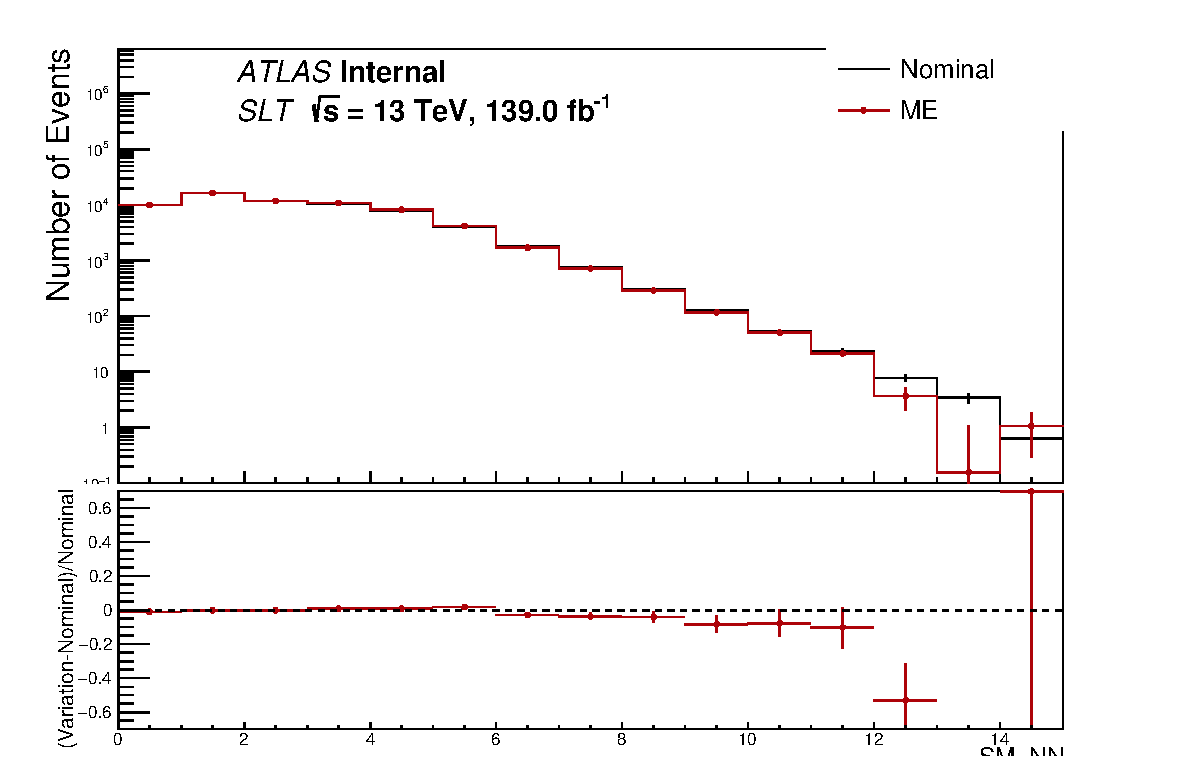
\includegraphics[width=.49\textwidth]{figures/lephad_modelling_systs/SLT/ME/limit_binning_SM_NN_Norm}
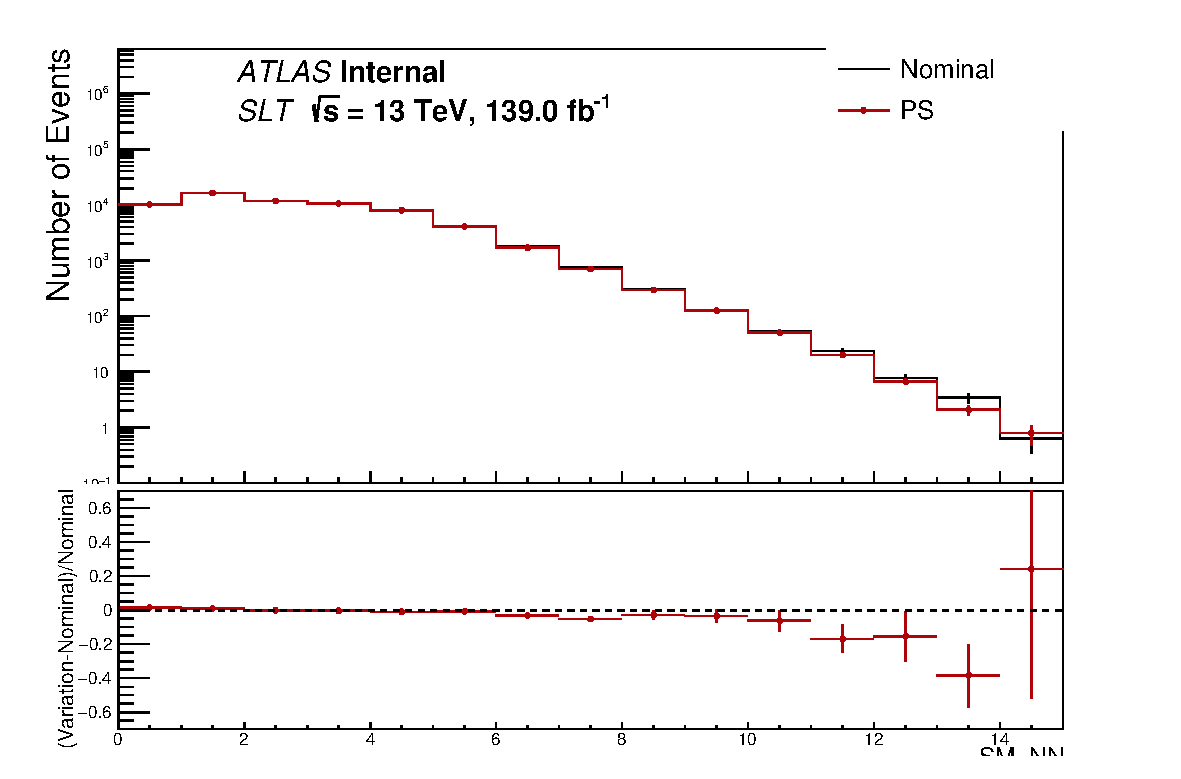
\includegraphics[width=.49\textwidth]{figures/lephad_modelling_systs/SLT/PS/limit_binning_SM_NN_Norm}\\
% 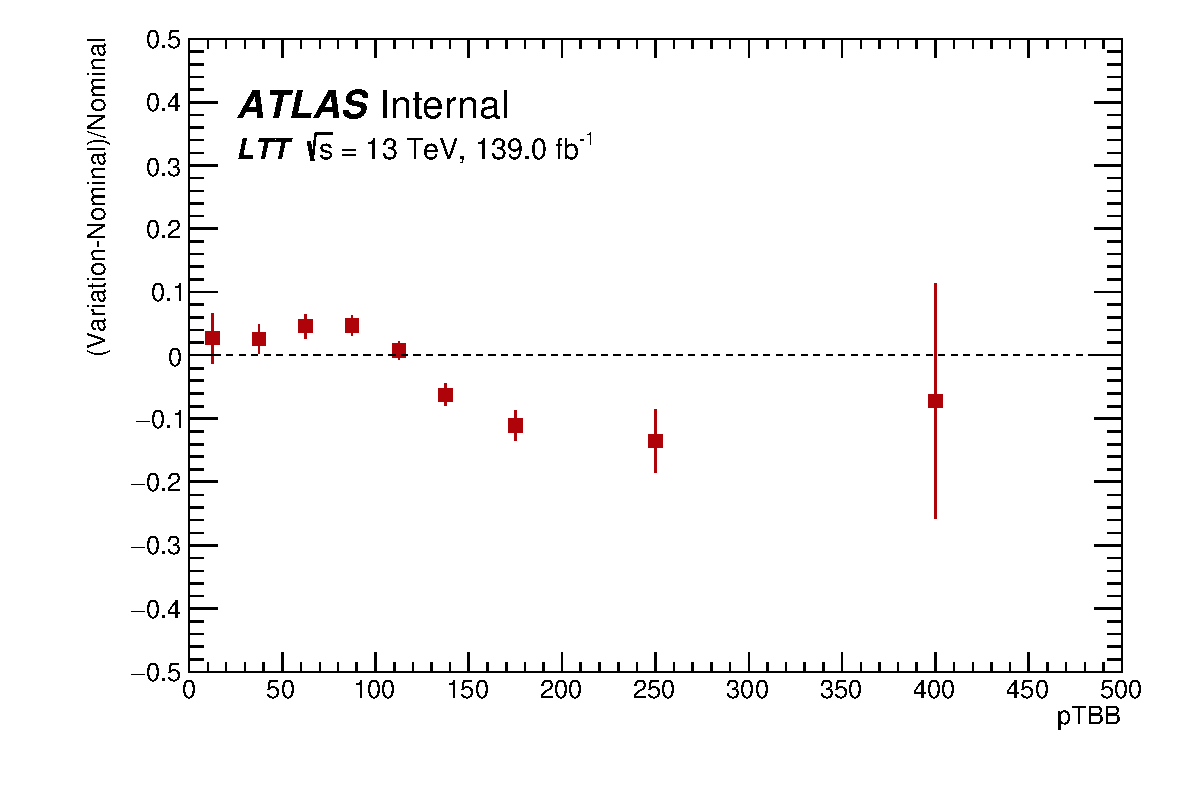
\includegraphics[width=.49\textwidth]{figures/lephad_modelling_systs/LTT/aMCNLO/pTBB_Norm}
% 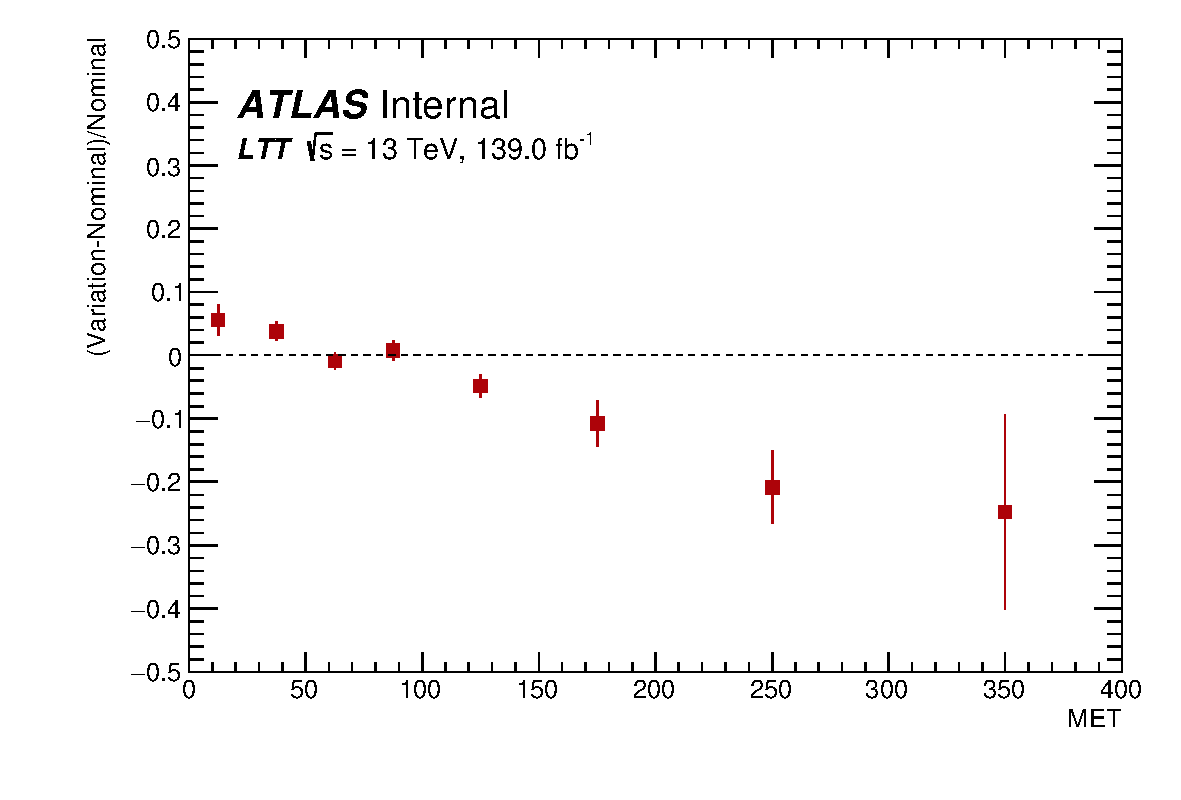
\includegraphics[width=.49\textwidth]{figures/lephad_modelling_systs/LTT/aMCNLO/MET_Norm}
\caption{Parametrisation in SM NN score distribution for the ME (left) and PS (right) systematics.}
\label{fig:ttbarsyst_lephad_SLT_NN}
\end{figure}


% \begin{figure}
%   \centering
%   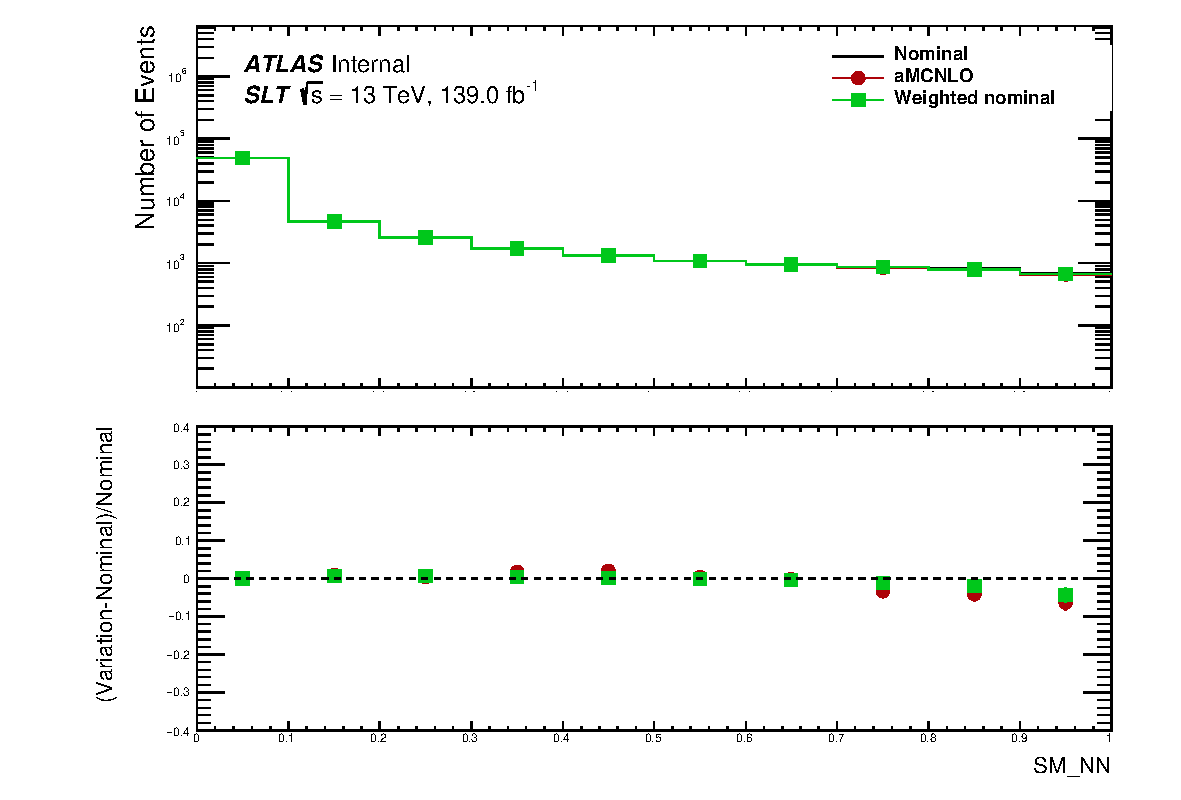
\includegraphics[width=.49\textwidth]{figures/lephad_modelling_systs/SLT/aMCNLO/Hist_and_ratio_SM_NN_Norm.png}
%   % 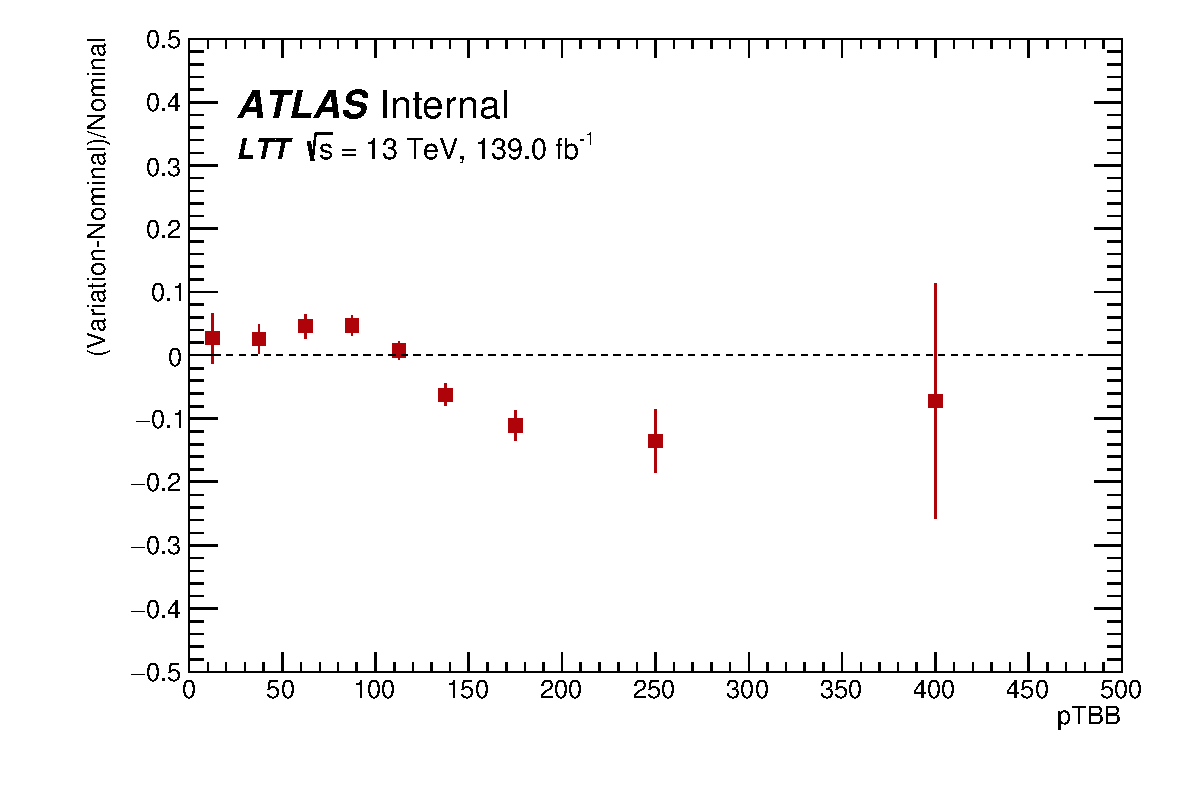
\includegraphics[width=.49\textwidth]{figures/lephad_modelling_systs/LTT/aMCNLO/pTBB_Norm.png}
%   % 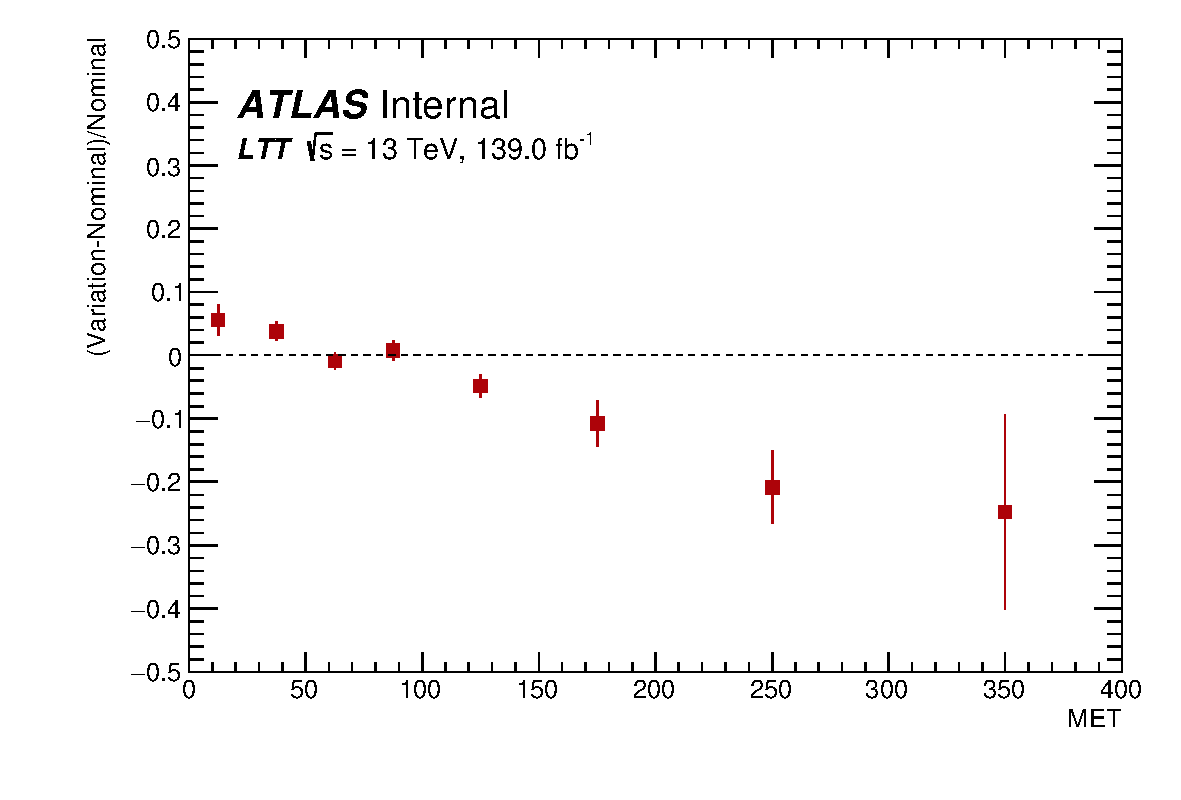
\includegraphics[width=.49\textwidth]{figures/lephad_modelling_systs/LTT/aMCNLO/MET_Norm.png}
%   \caption{SLT channel: shape-only NN score of the ME variation and the weighted nominal.}
%   \label{fig:ttbarsyst_lephad_amc_NN}
%   \end{figure}
  


%Parton shower hadronisation algorithmic uncertainties are evaluated comparing samples showered with Pythia8 versus Herwig7. 

% The parton shower uncertainty is parametrised similarly to the aMC 
% with a sequential parametrisation. The parametrisation is done first 
% in bins of the \pt\ of the subleading jet followed by parametrisation in bins
% of mass of the di-Higgs system, as shown in Fig.~\ref{fig:ttbarsyst_lephad_herwig}
% for the SLT channel. 
% The closure of the parametrisation in the NN score is shown in Fig.~\ref{fig:ttbarsyst_lephad_herwig_NN}.

% \begin{figure}
% 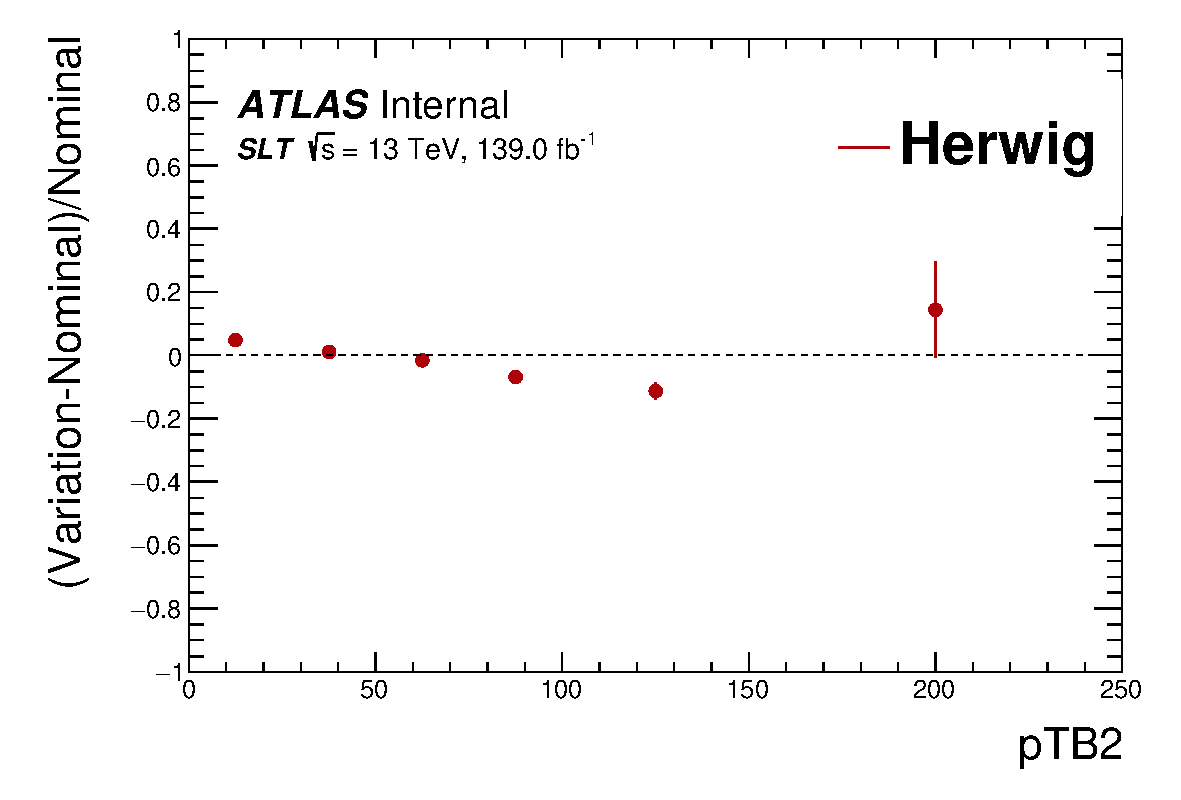
\includegraphics[width=.49\textwidth]{figures/lephad_modelling_systs/SLT/Herwig/pTB2_Norm.png}
% 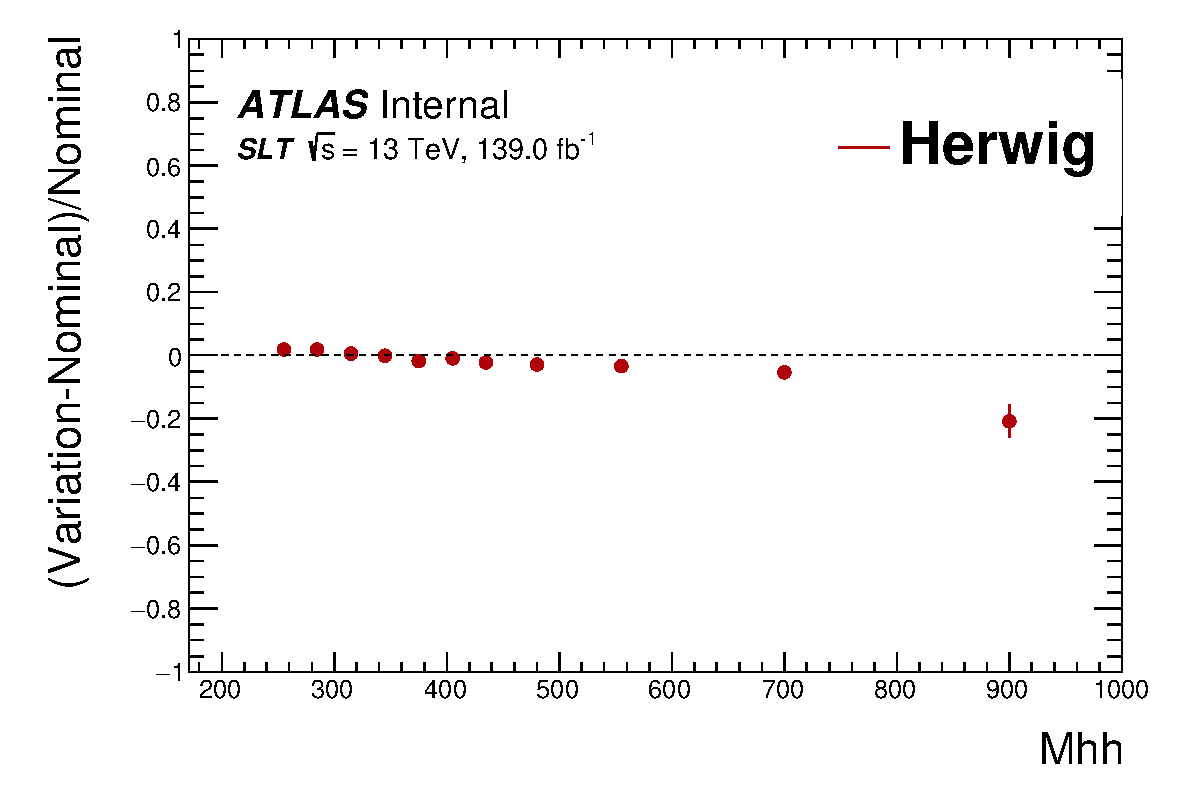
\includegraphics[width=.49\textwidth]{figures/lephad_modelling_systs/SLT/Herwig/Mhh_Norm.png}
% \caption{SLT: Parametrisation in bins of $p_T^{b2}$ distribution (left) and the $m_{HH}$ distribution
%  for the Herwig variation.}
% \label{fig:ttbarsyst_lephad_herwig}
% \end{figure}

% \begin{figure}
%   \centering
%   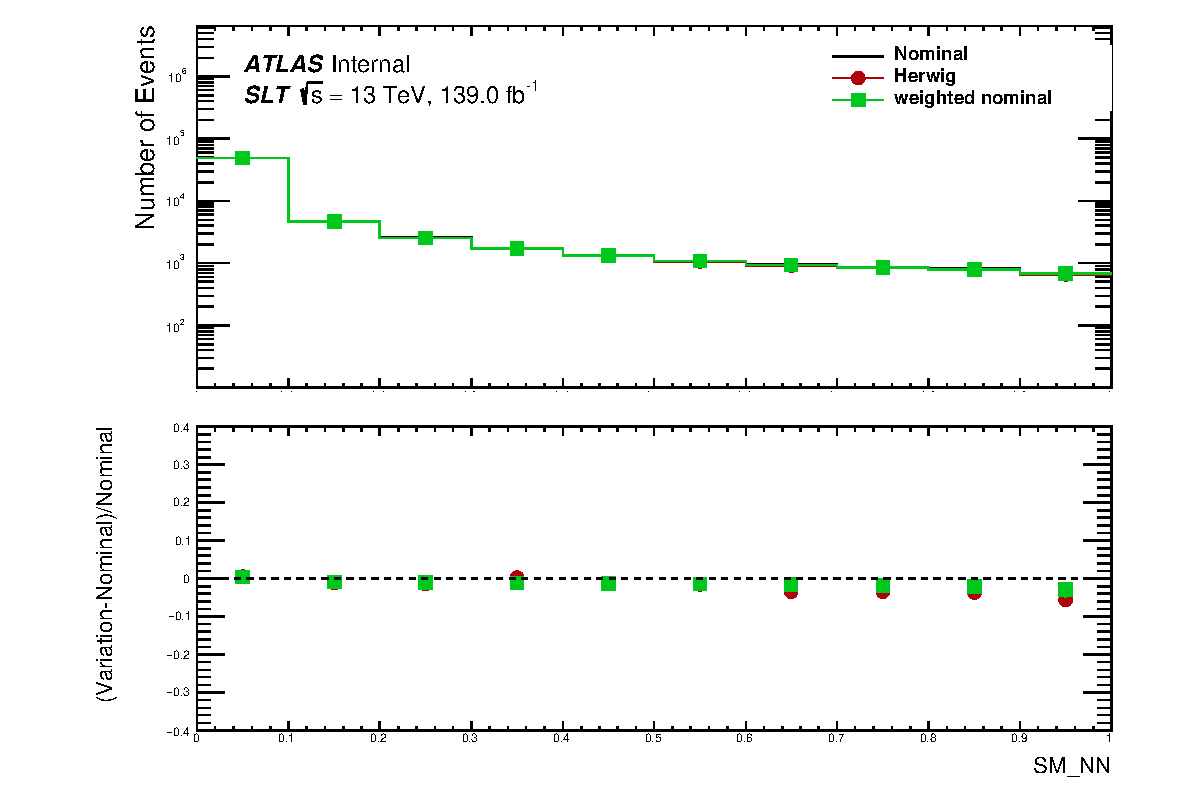
\includegraphics[width=.49\textwidth]{figures/lephad_modelling_systs/SLT/Herwig/Hist_and_ratio_SM_NN_Norm.png}
%   % 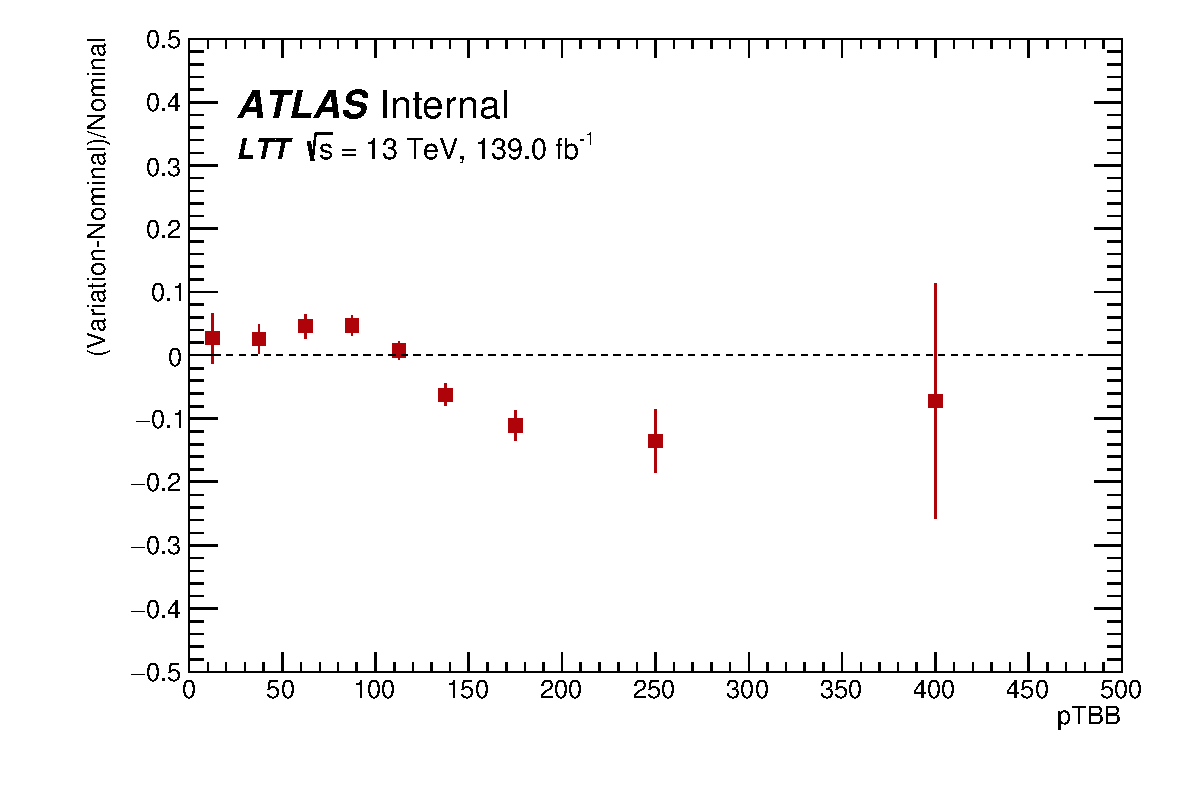
\includegraphics[width=.49\textwidth]{figures/lephad_modelling_systs/LTT/aMCNLO/pTBB_Norm.png}
%   % 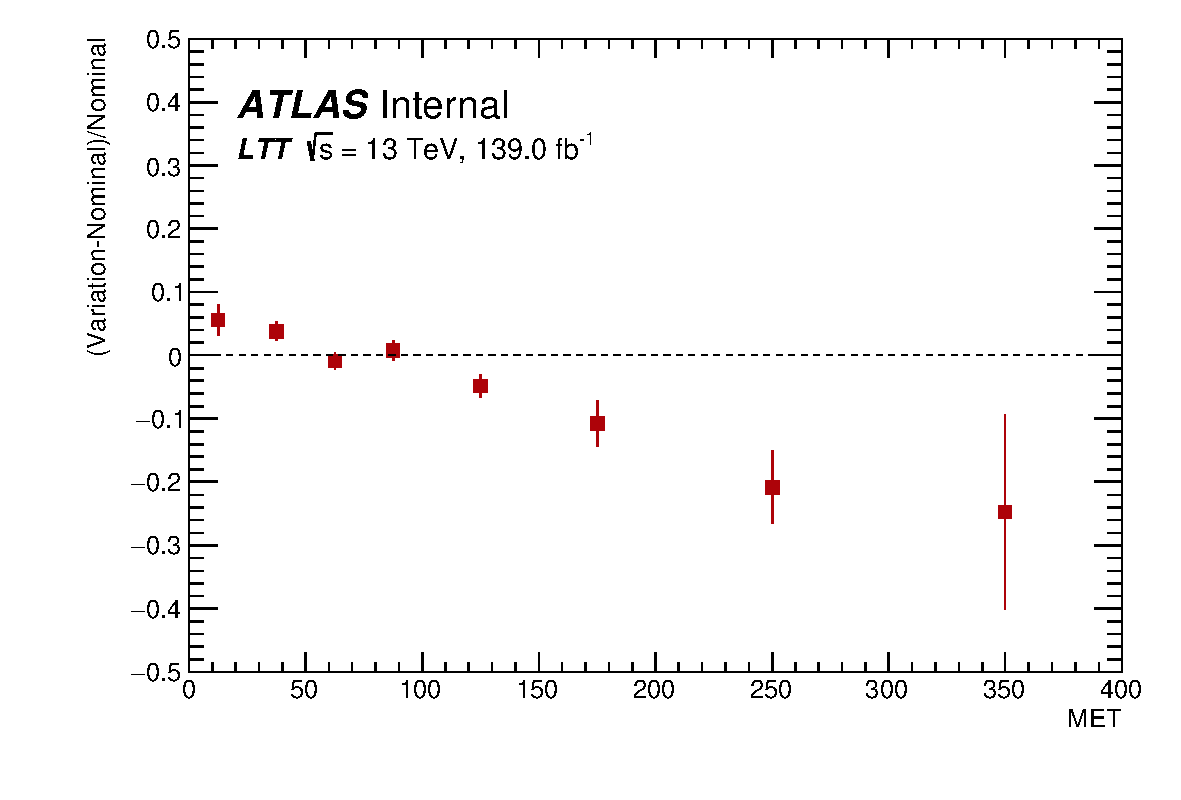
\includegraphics[width=.49\textwidth]{figures/lephad_modelling_systs/LTT/aMCNLO/MET_Norm.png}
%   \caption{SLT channel: shape-only NN score of the Herwig variation and the weighted nominal.}
%   \label{fig:ttbarsyst_lephad_herwig_NN}
%   \end{figure}
  

The ISR up and down variations have not shown obvious shape in the NN/PNN distribution 
therefore only normalisation uncertainty is considered. 
%  \begin{figure}
% \centering
% 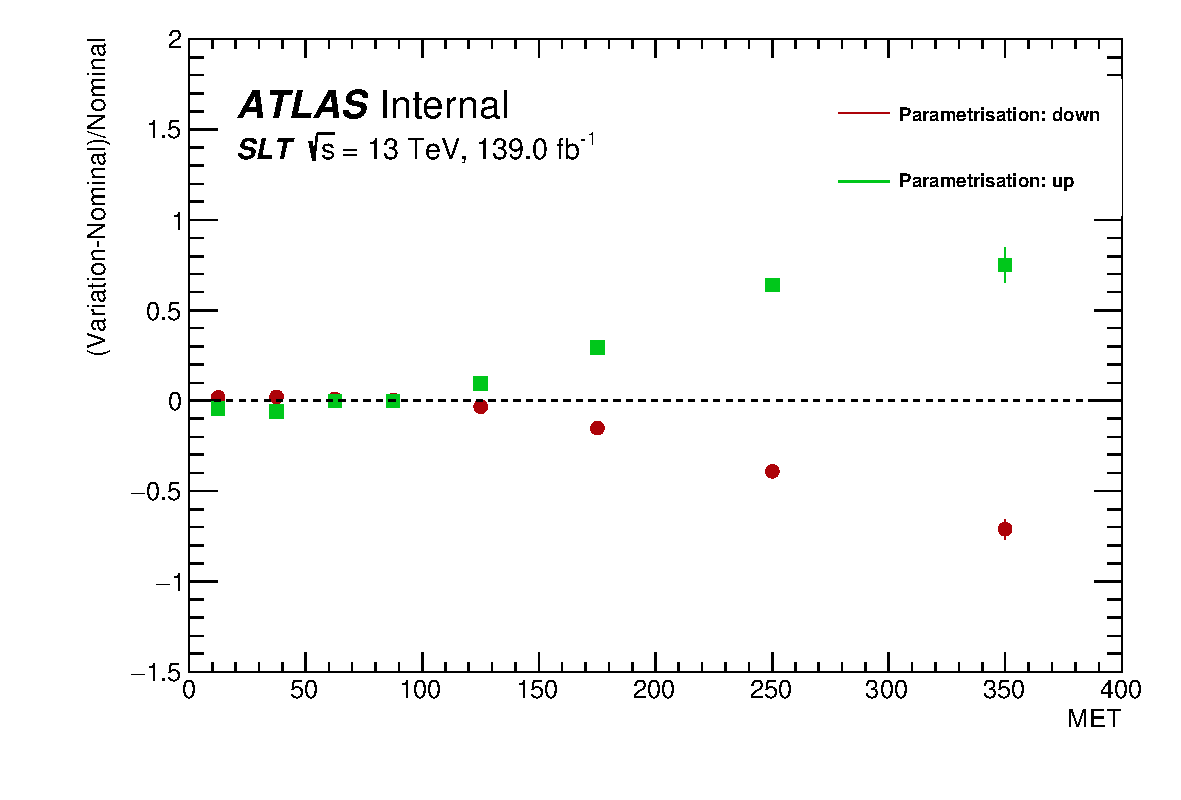
\includegraphics[width=.49\textwidth]{figures/lephad_modelling_systs/SLT/ISRlow/MET_Norm.png}
% 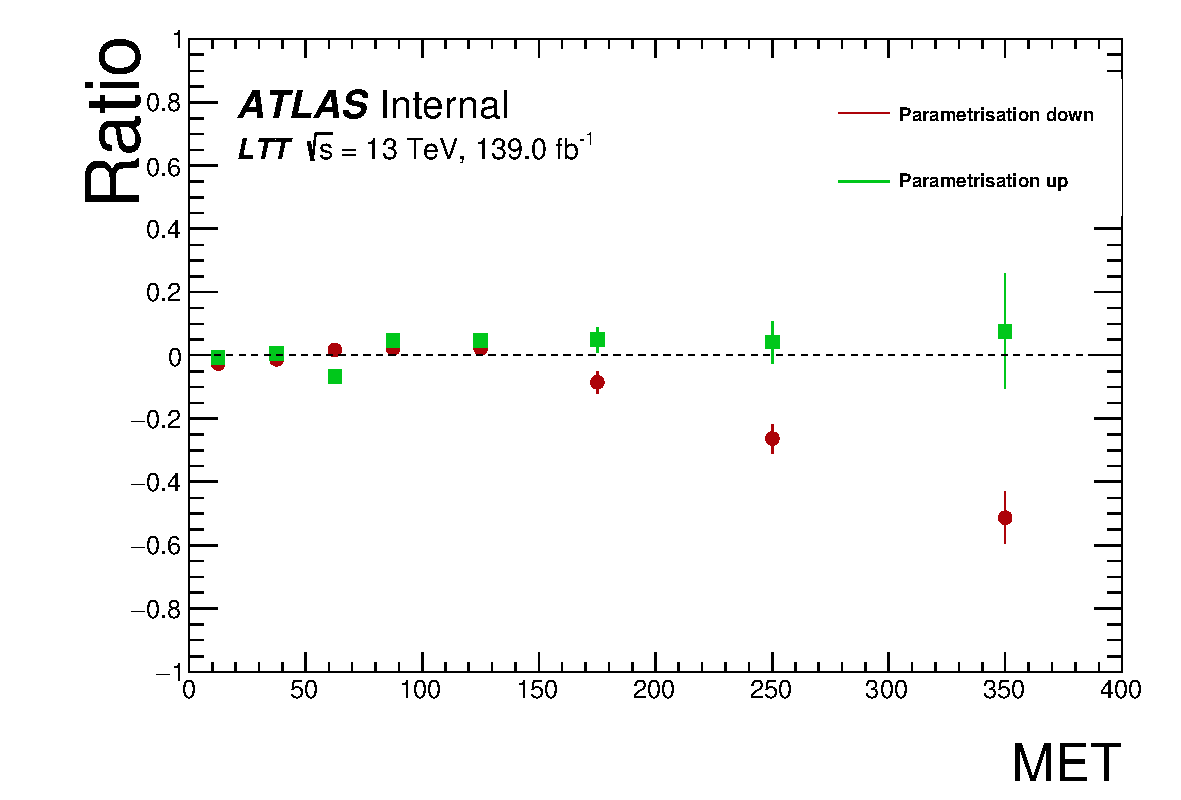
\includegraphics[width=.49\textwidth]{figures/lephad_modelling_systs/LTT/ISRlow/MET_Norm.png}
% \caption{SLT (left) and LTT channel (right): Parametrisation in bins of the MET distribution for the ISR variation.}
% \label{fig:ttbarsyst_lephad_isr_MET}
% \end{figure}





\paragraph{Uncertainties on $t\bar{t}$ in the \hadhad
  channel}\mbox{}\\

The shapes of two-point \ttbar modelling uncertainties (i.e.\ ME, PS
and ISR) are directly estimated by comparing the MVA discriminants of
the (fast-sim.) variation sample with the nominal (fast-sim.) \ttbar
sample. The shape differences are parametrized by taking the ratio of
the normalized variation histogram and the normalized nominal
histogram in bins of the MVA discriminant. This ratio is subsequently
applied as a multiplicative factor to the nominal \ttbar sample using
full simulation. To limit the impact of statistical fluctuations on
the variation template entering the fit, the binning of the ratio
parametrizing the shape is chosen such that about 5 \% of nominal
\ttbar populates each bin\footnote{The exact fraction can vary as the
  derivation is performed using pre-binned data using the same binning
  that is also used as the input to the rebinning algorithms used in
  the final fit. In extreme cases, e.g.\ for the high-mass PNN
  discriminants, where almost perfect discrimination between signal
  and \ttbar is possible the exact fraction can be significantly
  larger.}. This limits the statistical uncertainties on the weighting
factors describing the shape of the uncertainty to less than 3 \% and
allows for a good description of the bulk of \ttbar events.

In~\ref{fig:hadhad_ttbar_syst_parametrization} the parametrization of
the \ttbar ME, PS and ISR uncertainties is shown with respect to the
SM-BDT. The parametrization for all PNN distributions is done
analogously. The main difference of the PNN parametrization is that
for the PNN discriminants used to extract high-mass resonances, the
high MVA-score region is dominated by the Z+jets background and close
to perfect discrimination between signal and \ttbar discrimination is
possible. Therefore, \ttbar is concentrated in the first bin of the
fitted distributions leading to no sensitivity to shape differences of
the MVA distribution for \ttbar.

\begin{figure}[htbp]
  \centering

  \subfloat[]{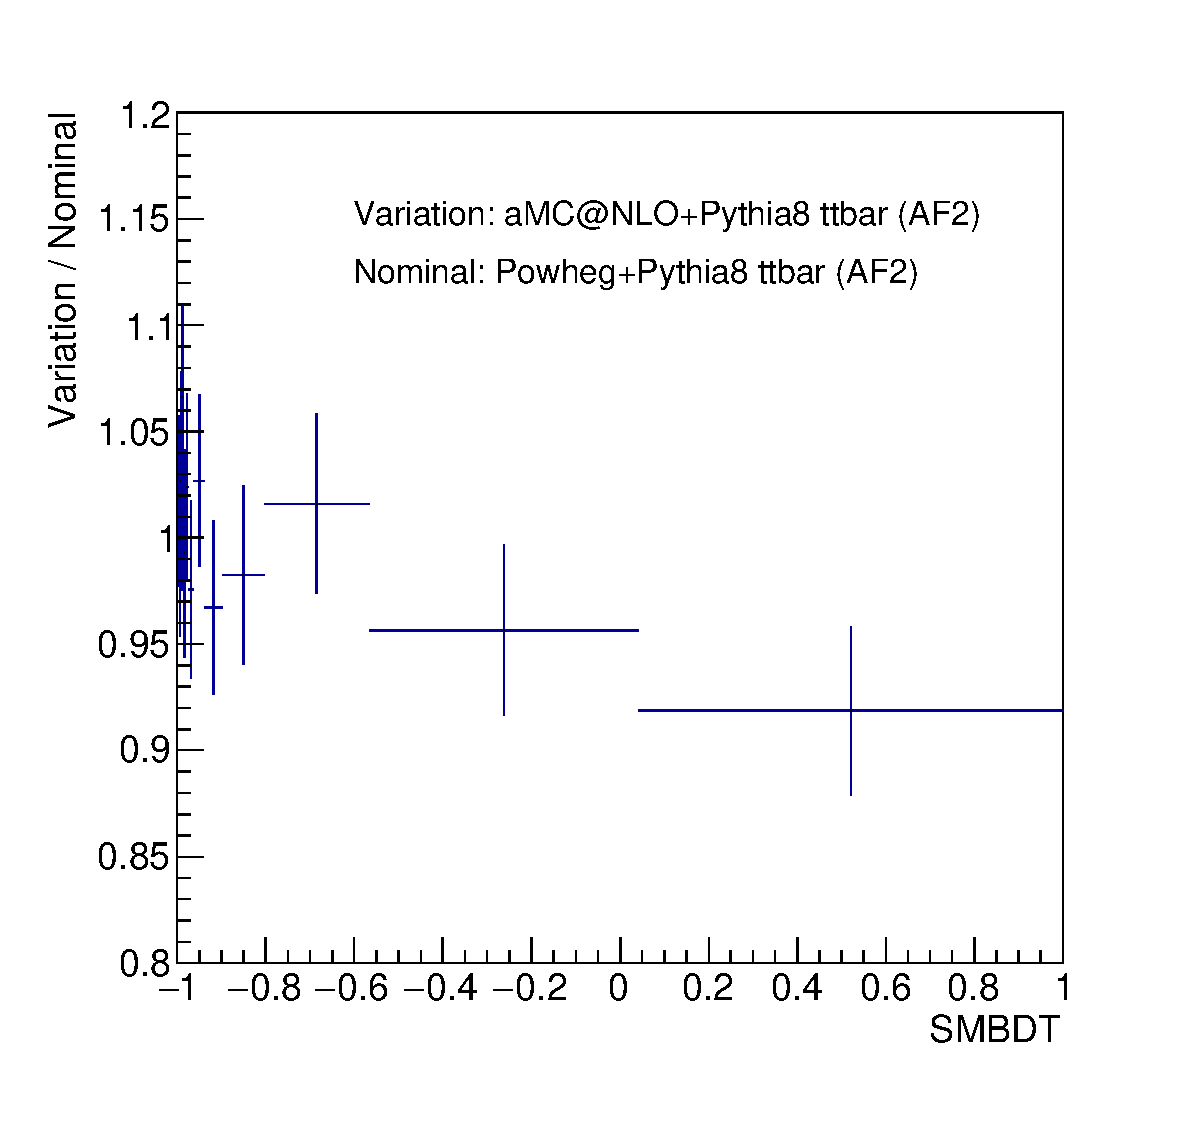
\includegraphics[width=0.33\textwidth]{figures/systs/hadhad_ttbar/hadhad_ttbar_me_mvaparam_SMBDT}}
  \subfloat[]{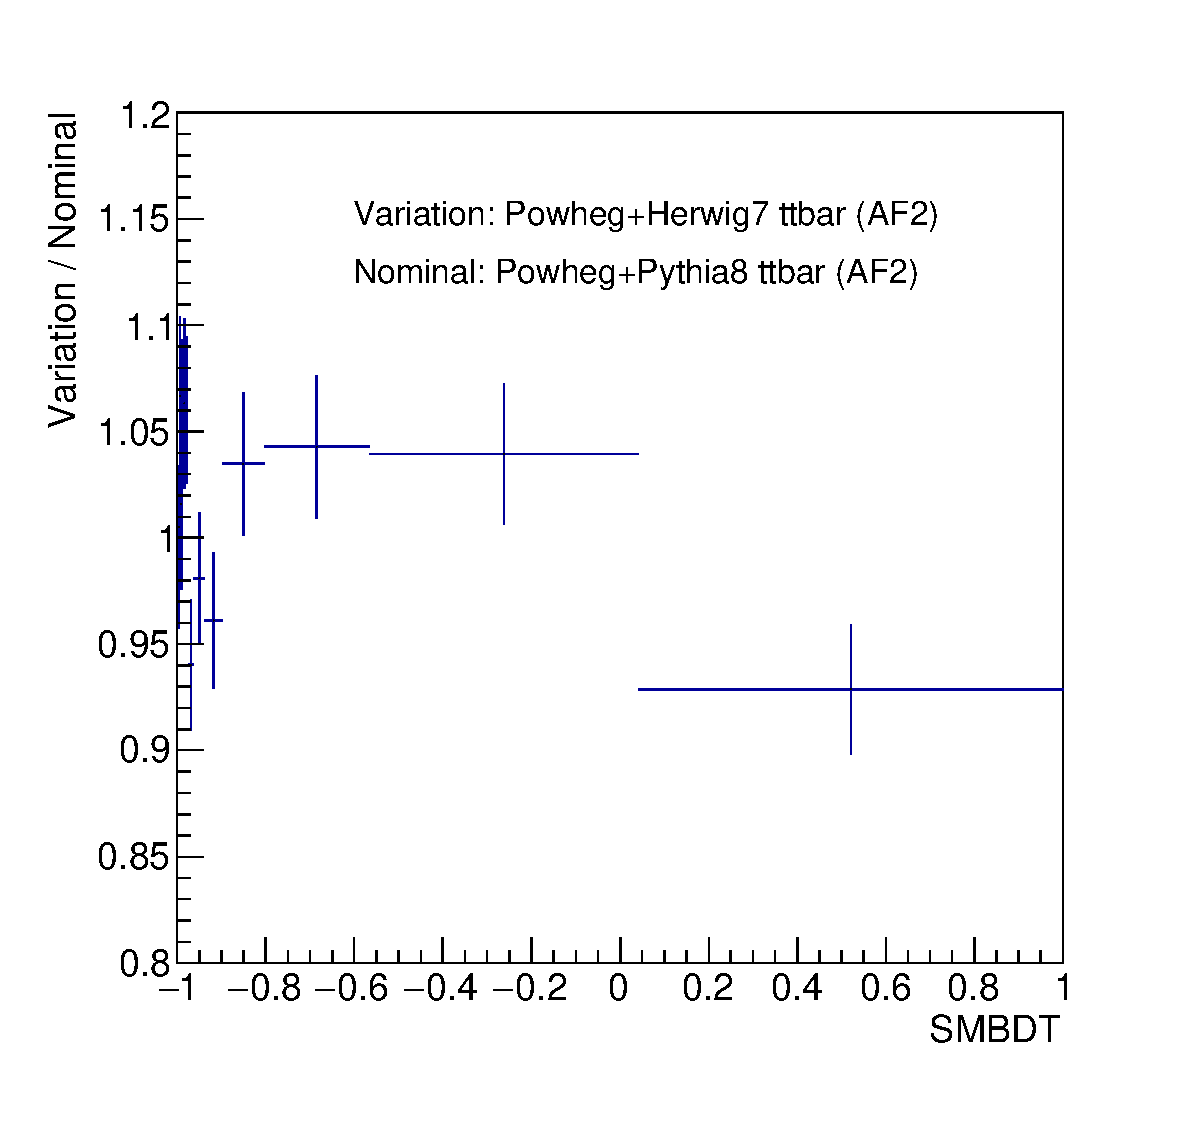
\includegraphics[width=0.33\textwidth]{figures/systs/hadhad_ttbar/hadhad_ttbar_ps_mvaparam_SMBDT}}
  \subfloat[]{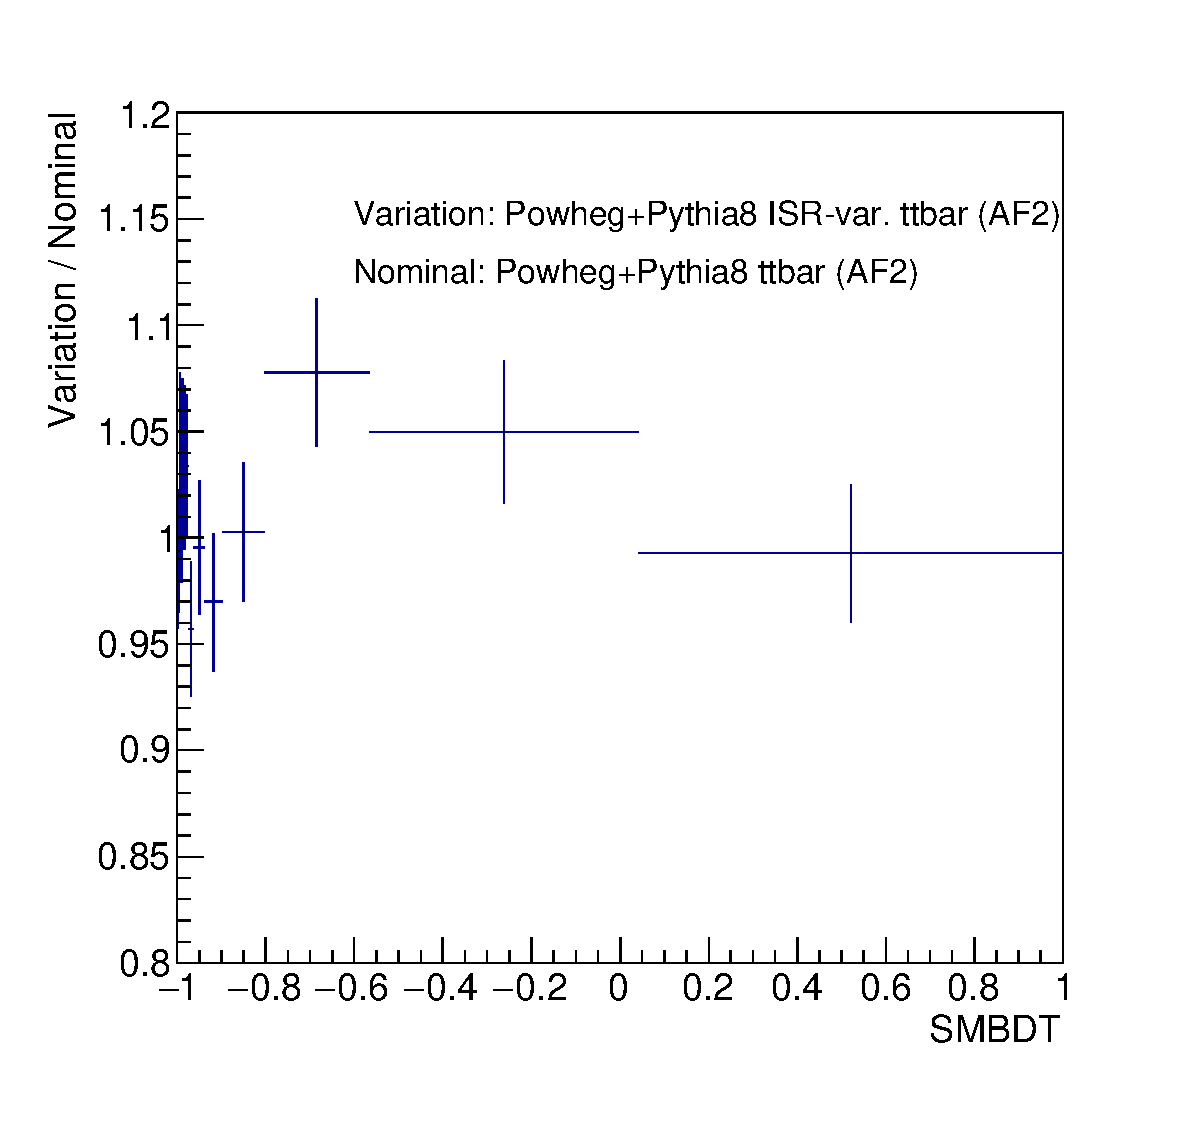
\includegraphics[width=0.33\textwidth]{figures/systs/hadhad_ttbar/hadhad_ttbar_isr_mvaparam_SMBDT}}

  \caption{Parametrization of the generator (a), parton shower (b) and
    ISR uncertainty (c) for the SMBDT distribution.}
  \label{fig:hadhad_ttbar_syst_parametrization}
\end{figure}

In~\ref{fig:hadhad_ttbar_syst_closure} the closure of the
parametrized uncertainties is shown for the SMBDT. The full set of all
relevant distributions is shown
in~\ref{subsec:appendix_systs_ttbarsysts_hadhad}.


\begin{figure}[htbp]
  \caption{Closure check of parametrized \ttbar uncertainties in the
    \hadhad channel for the generator (ME), parton shower (PS) and ISR
    uncertainty. The binning used for the closure check is the same as
    used for the final signal extraction fit. Note: The x-axis does
    not directly correspond to what is shown 
    in~\ref{fig:hadhad_ttbar_syst_parametrization} but uses the
    convention used for the final fit.}
  \label{fig:hadhad_ttbar_syst_closure}
\end{figure}

% Due to poor statistical precision of samples used for estimating \ttbar
% modelling uncertainties at high MVA score in $\tauhad\tauhad$, shape
% uncertainties are parametrised in other observables of the event and
% subsequently applied to the nominal \ttbar sample.

% The variation of the matrix element is parametrised in bins of the \pT of the
% \ttbar system. Residual variations (after \pT-\ttbar reweighting) are then
% evaluated in bins of the \pT of the subleading top. The parametrisation is shown
% in~\ref{fig:ttbarsyst_hadhad_me}.

% \begin{figure}
%   \centering
% 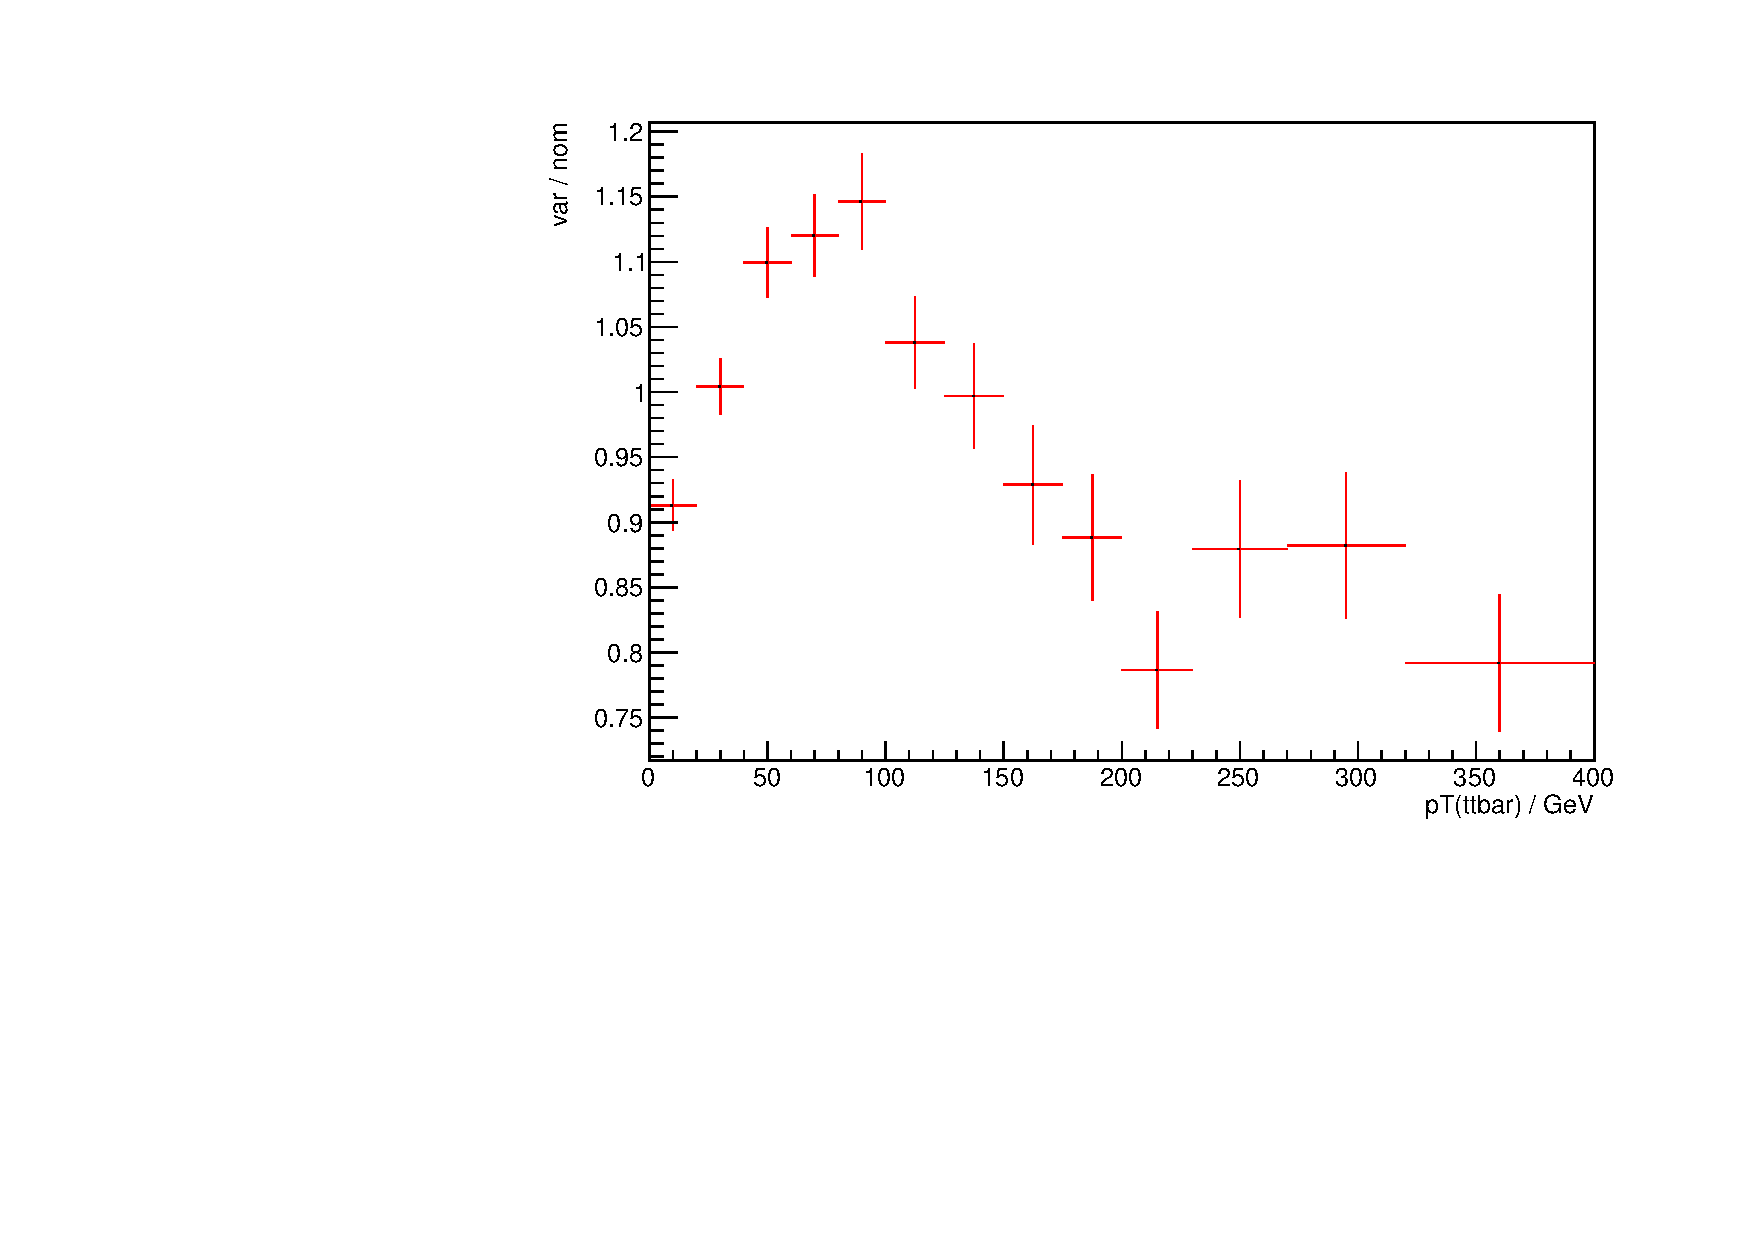
\includegraphics[width=0.49\textwidth]{figures/systs/hadhad_ttbar/me_ttbarpt}
% 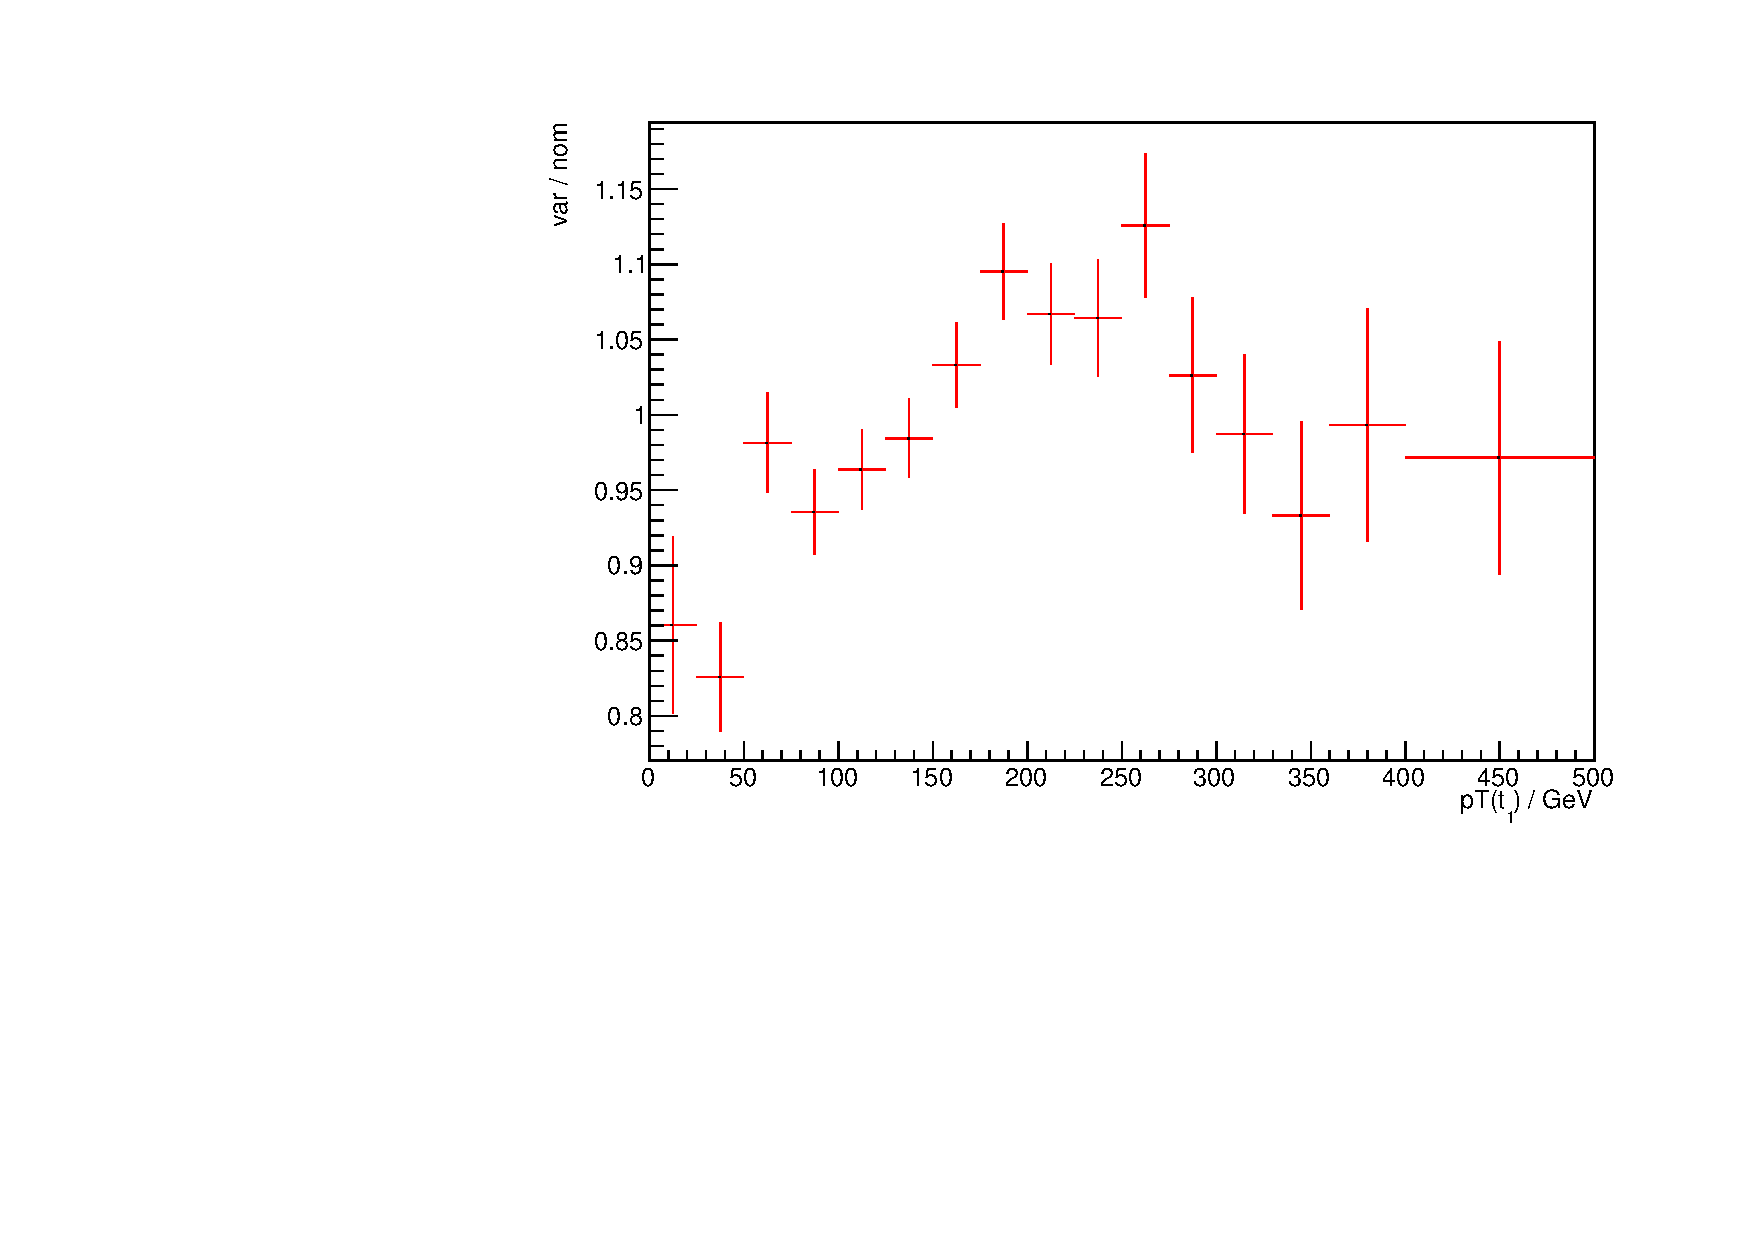
\includegraphics[width=0.49\textwidth]{figures/systs/hadhad_ttbar/me_toppt}
%   \caption{Parametrisation of the matrix element uncertainty (aMCAtNLO) in
%     $\tauhad\tauhad$. The ratio of variation and nominal yield is parametrised in bins of truth
%     \pT of the \ttbar system and truth \pT of the subleading top.}
%   \label{fig:ttbarsyst_hadhad_me}
% \end{figure}

% Similarly, the uncertainty due to the choice of parton shower is estimated by
% comparing Herwig7 with Pythia8. The uncertainty is parametrised sequentially in
% the leading and subleading b-jet \pT without applying any b-jet energy
% corrections. The parametrisation is shown in Figure~\ref{fig:ttbarsyst_hadhad_ps}.



% \begin{figure}
%   \centering
% 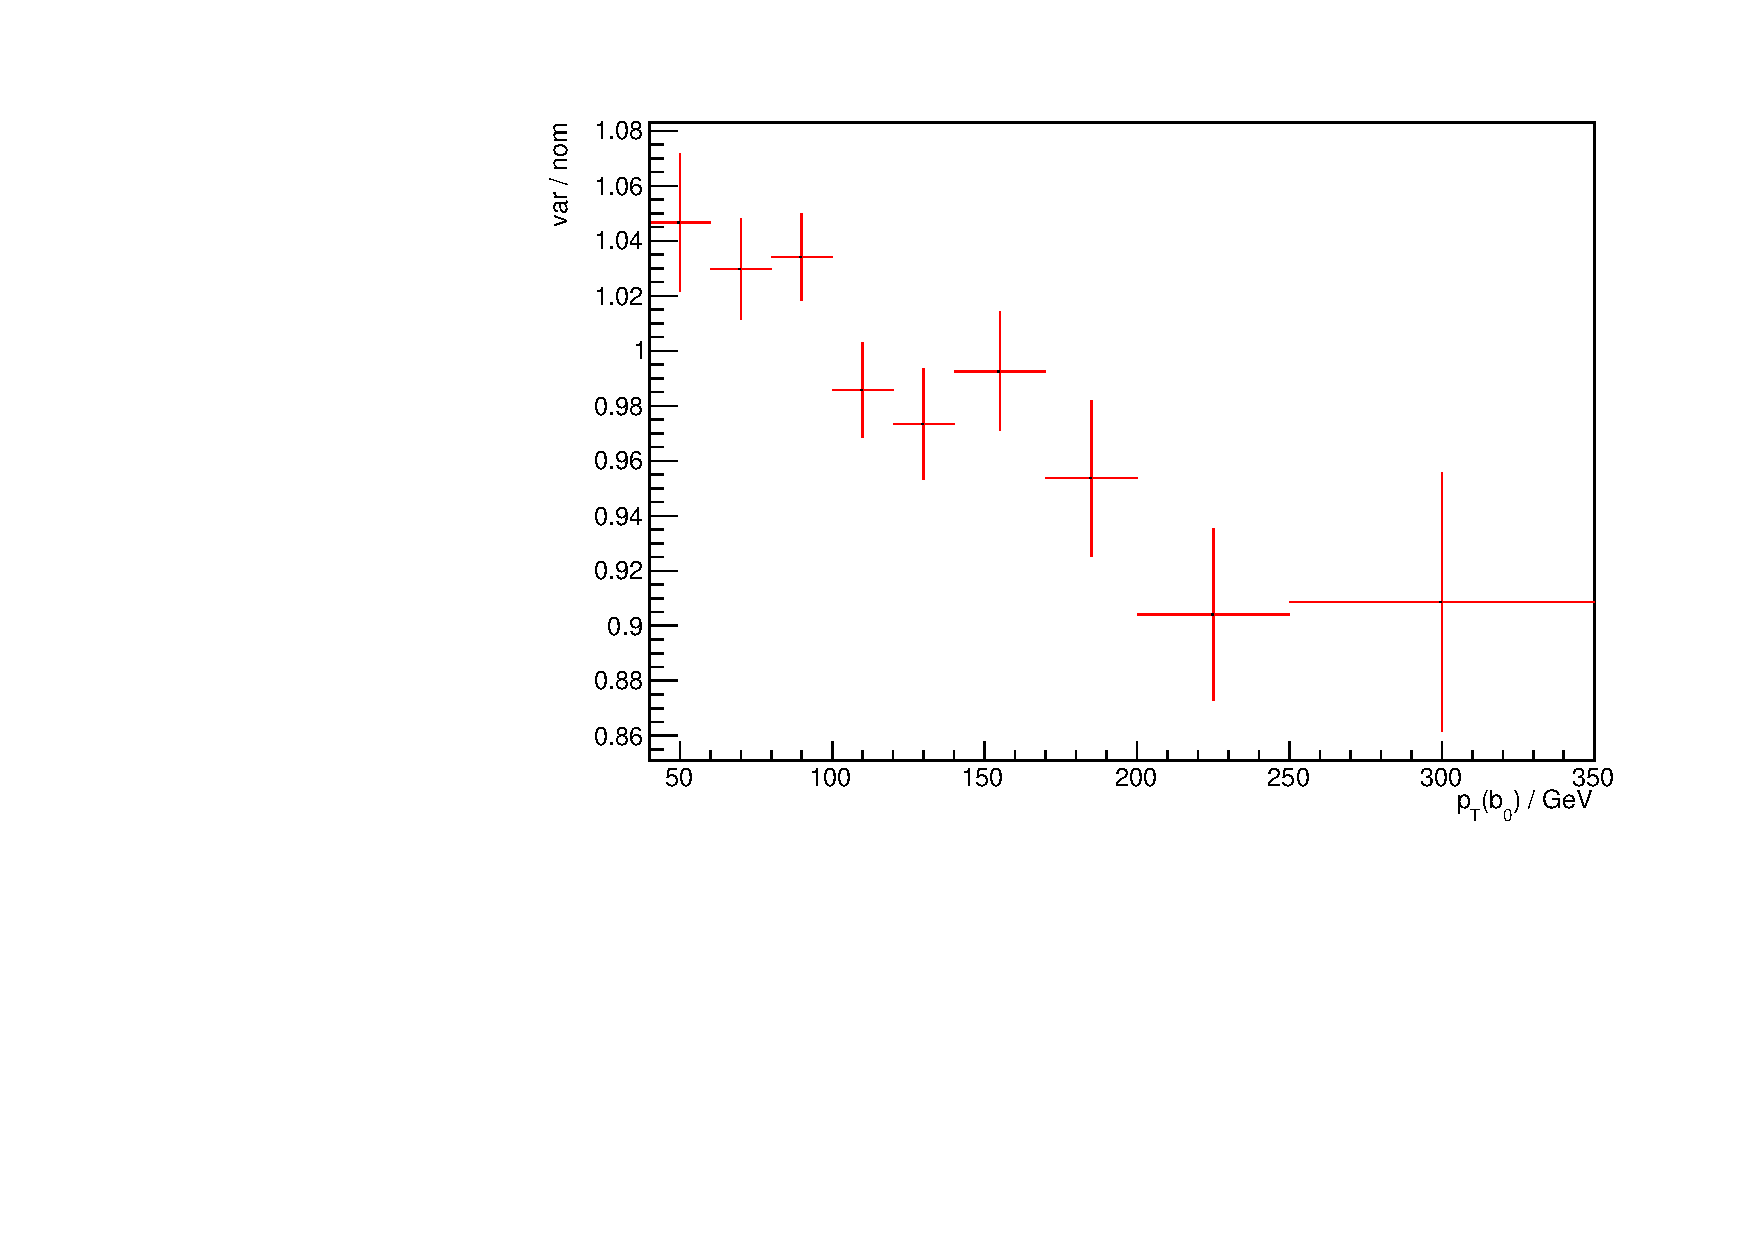
\includegraphics[width=0.49\textwidth]{figures/systs/hadhad_ttbar/ps_b0pt}
% 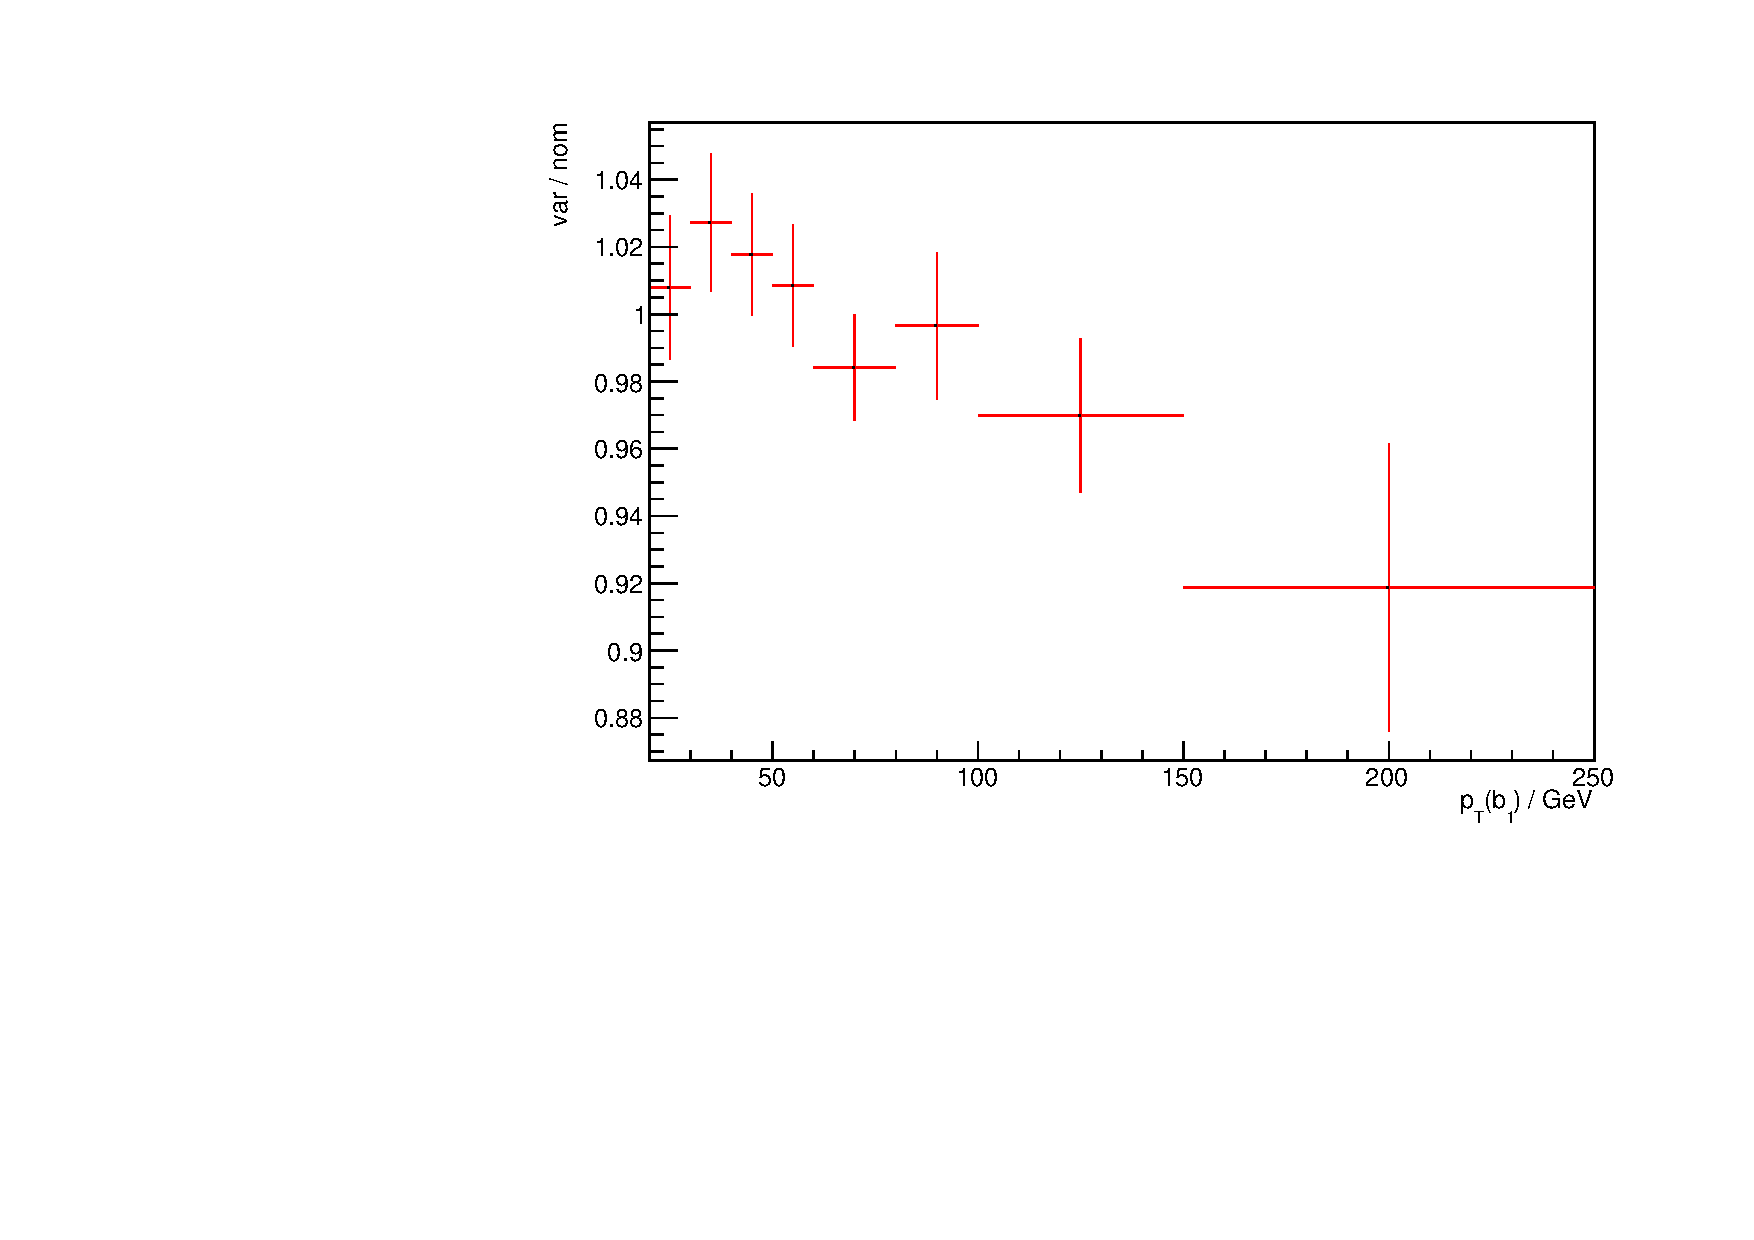
\includegraphics[width=0.49\textwidth]{figures/systs/hadhad_ttbar/ps_b1pt}
%   \caption{Parametrisation of the parton shower uncertainty (Herwig7) in
%     $\tauhad\tauhad$. The ratio of variation and nominal yield is parametrised in bins fo leading
%     and subleading b-jet \pT (before b-jet corrections).}
%   \label{fig:ttbarsyst_hadhad_ps}
% \end{figure}

% The modelling uncertainty due to initial state radiation is sequentially
% parametrized in the number of jets at truth-level with at least $\pT >
% \SI{20}{\GeV}$ and the \pT of the \ttbar-system. The parametrisation is shown in Figure~\ref{fig:ttbarsyst_hadhad_isr}.

% \begin{figure}
%   \centering
% 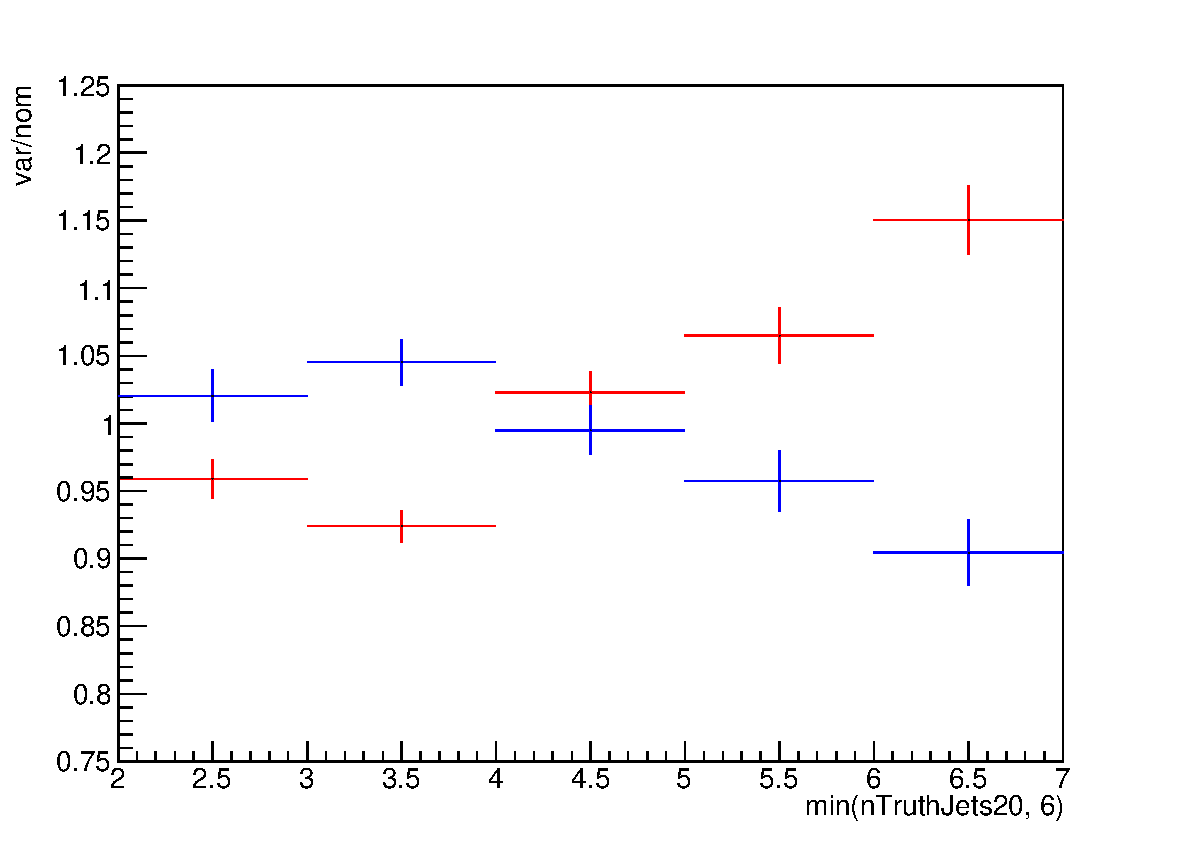
\includegraphics[width=0.49\textwidth]{figures/systs/hadhad_ttbar/isr_njets}
% 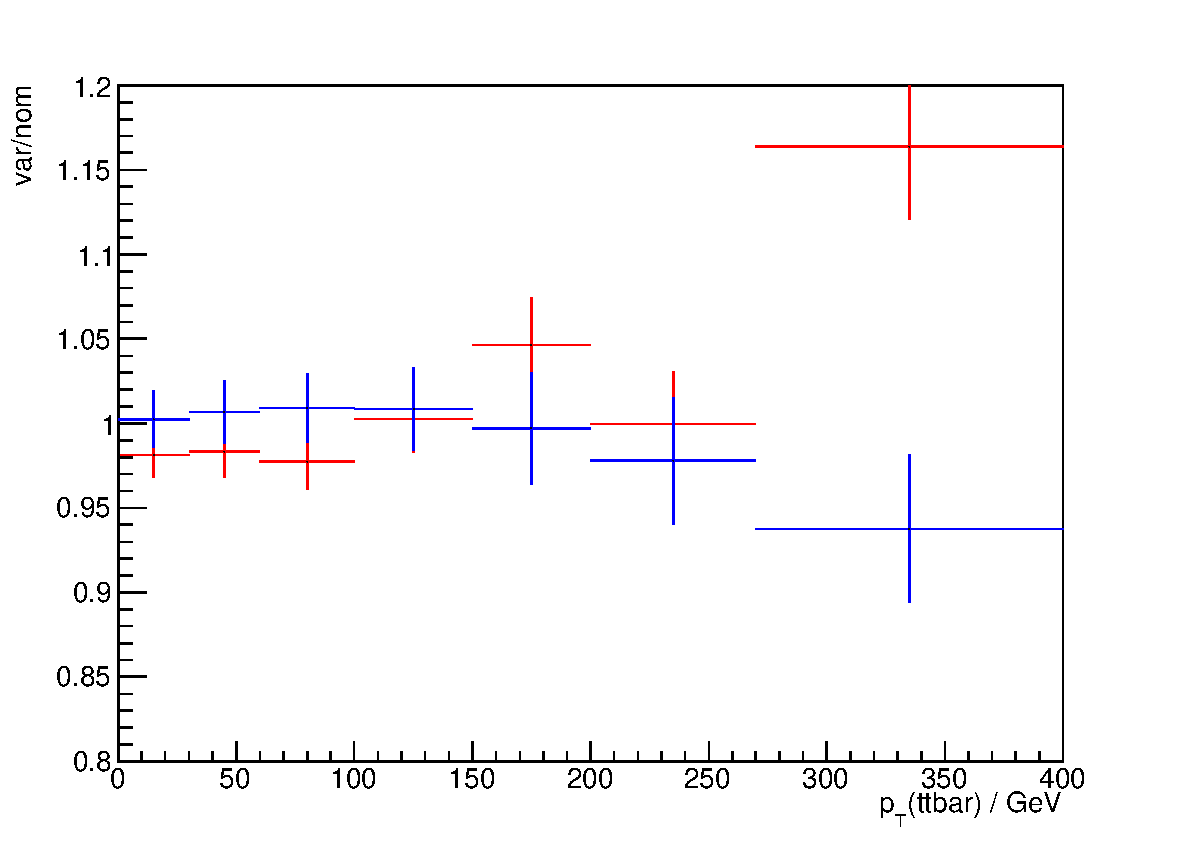
\includegraphics[width=0.49\textwidth]{figures/systs/hadhad_ttbar/isr_ttbarpt}
%   \caption{Parametrisation of the ISR uncertainty in $\tauhad\tauhad$ (up
%     variation in red, down variation in blue). The ratio
%   of variation and nominal yield is parametrised in bins of the number of truth
%   jets ($\pT > \SI{20}{\GeV}$) and \pT of the \ttbar system.}
%   \label{fig:ttbarsyst_hadhad_isr}
% \end{figure}

% The validity of the above parametrisations is examined by applying the
% parametrisation on the nominal \ttbar sample and comparing the MVA-score
% distributions used for signal extraction between the reweighted nominal and the
% variation. An exemplary closure check for the \SI{500}{\GeV} PNN-score
% distribution can be found in~\ref{fig:ttbarsyst_hadhad_closure}.

% \begin{figure}
%   \centering
% 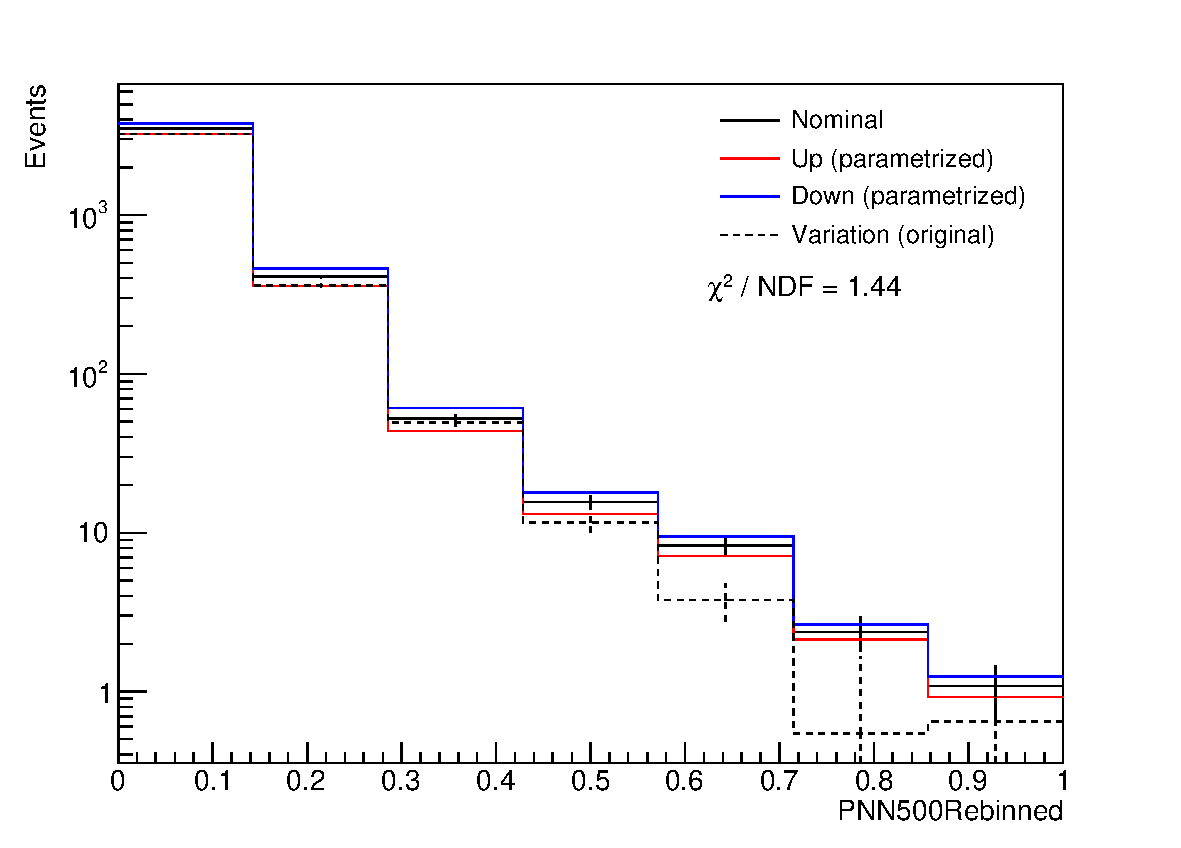
\includegraphics[width=0.32\textwidth]{figures/systs/hadhad_ttbar/gen_pnn500}
% 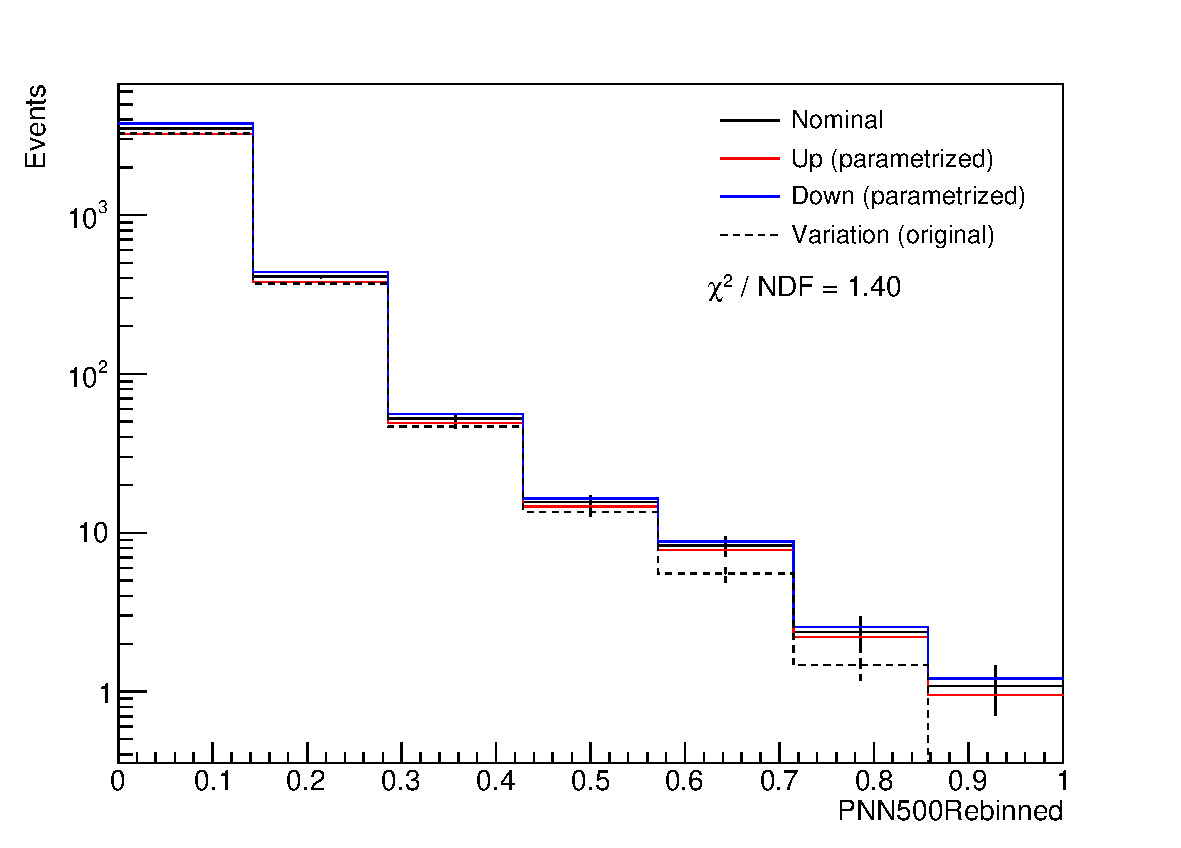
\includegraphics[width=0.32\textwidth]{figures/systs/hadhad_ttbar/ps_pnn500}
% 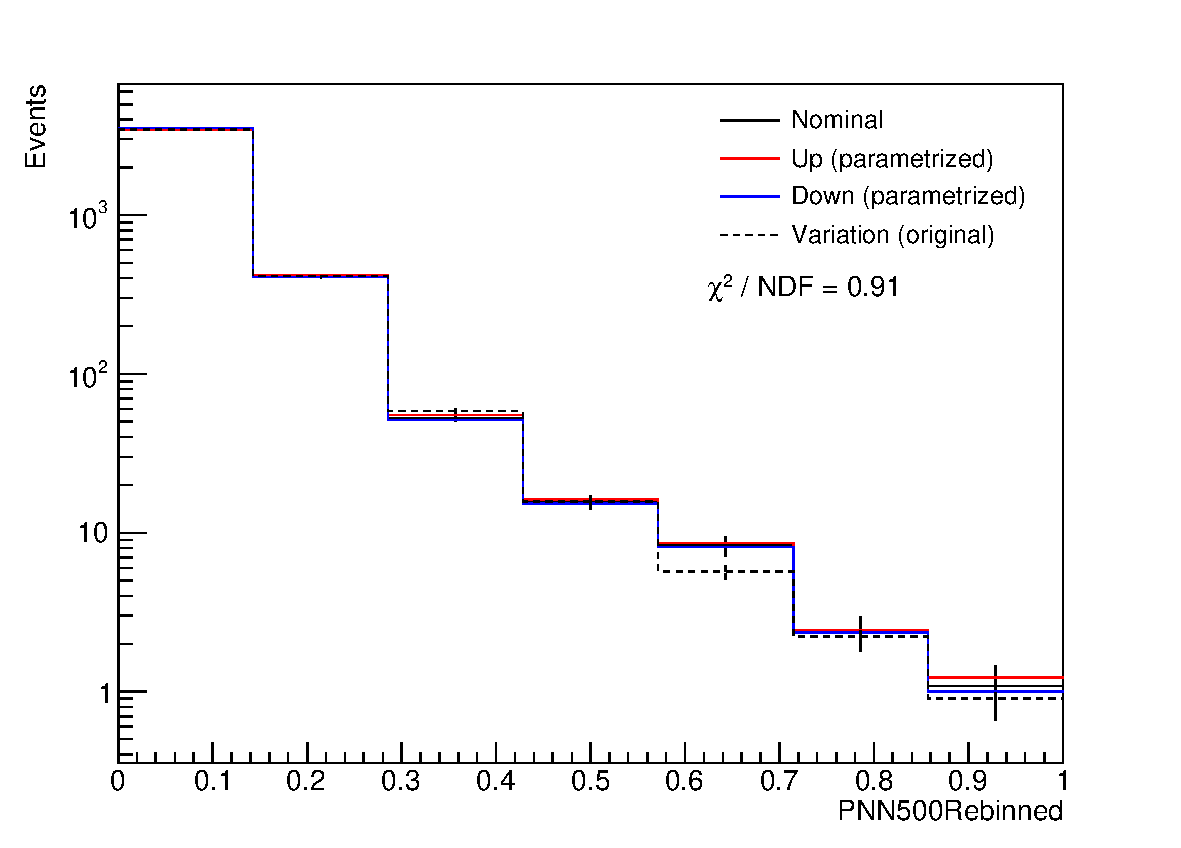
\includegraphics[width=0.32\textwidth]{figures/systs/hadhad_ttbar/isr_pnn500_up}
%   \caption{Closure check of $\tauhad\tauhad$ matrix element (left), parton shower
%     (middle) and ISR uncertainty (right) in the PNN500 distribution used to extract the
%     $X(500) \to b\bar{b}\tauhad\tauhad$ signal.}
%   \label{fig:ttbarsyst_hadhad_closure}
% \end{figure}

% The parametrizations are then passed through the PNN classification, and the resulting variations are shown in Appendix~\ref{subsec:appendix_systs_ttbarsysts_hadhad}.

\paragraph{Uncertainties on $t\bar{t}$ in the Z+HF control region}\mbox{}\\

Shape uncertainties on the $t\bar{t}$ background are neglected in the Z+HF 
control region as they are found to be negligible in the $m_{\ell\ell}$ distribution included in the fit for this region, as shown in Appendix~\ref{subsec:appendix_systs_ttbarsysts_ZCR}.
